% ============================================================
%  Entropy Box: A Knowledge Compiler for Embodied AI
%  arXiv system paper -- LaTeX source
%  Compile: pdflatex main && pdflatex main
% ============================================================
\documentclass[10pt,a4paper]{article}

\usepackage[margin=0.95in]{geometry}
\usepackage[T1]{fontenc}
\usepackage[utf8]{inputenc}
\usepackage{lmodern}
\usepackage{amsmath,amssymb}
\usepackage{booktabs}
\usepackage{graphicx}
\usepackage{xcolor}
\usepackage{tikz}
\usetikzlibrary{arrows.meta,positioning,shapes.geometric,fit,backgrounds,calc}
\usepackage{caption}
\usepackage{subcaption}
\usepackage{enumitem}
\usepackage{microtype}
\usepackage{multirow}
\usepackage{pgfplots}
\pgfplotsset{compat=1.16}
\usepackage{authblk}
\usepackage[hidelinks,breaklinks]{hyperref}
\usepackage{url}

\captionsetup{font=small,labelfont=bf}

\definecolor{ebblue}{HTML}{1F4E79}
\definecolor{ebteal}{HTML}{2E7D7B}
\definecolor{ebamber}{HTML}{B7791F}
\definecolor{ebgray}{HTML}{F2F4F7}
\definecolor{ebline}{HTML}{9AA5B1}

\newcommand{\eb}{\textsc{Entropy Box}\xspace}
\usepackage{xspace}

\tikzset{
  block/.style={rectangle, rounded corners=2pt, draw=ebline, fill=ebgray,
                align=center, font=\small, minimum height=8mm, inner sep=4pt},
  gate/.style={rectangle, rounded corners=2pt, draw=ebamber, fill=ebamber!10,
               align=center, font=\small, minimum height=8mm, inner sep=4pt},
  store/.style={rectangle, rounded corners=2pt, draw=ebteal, fill=ebteal!10,
                align=center, font=\small, minimum height=8mm, inner sep=4pt},
  hdr/.style={rectangle, rounded corners=2pt, draw=ebblue, fill=ebblue!12,
              align=center, font=\small\bfseries, minimum height=8mm, inner sep=4pt},
  ar/.style={-{Stealth[length=2mm]}, draw=ebline, thick},
}

% ------------------------------------------------------------
\title{\vspace{-1.2cm}\textbf{Entropy Box: A Knowledge Compiler for Embodied AI}\\[0.35em]
\large Towards Structured Knowledge Compilation for Robotics Foundation Models}

\author{Yuqi Wang}
\affil{\small Entropy Box\\
\texttt{wangyuqi11and11@163.com} \quad\textbullet\quad \url{https://chenli-yy.github.io/entropy-box-public/}}
\date{\today}

\begin{document}
\maketitle

% ============================================================
\begin{abstract}
\noindent
The bottleneck in embodied AI today is not model capacity --- it is knowledge.
The engineering knowledge a robot needs already exists: in tens of thousands of
papers, GitHub repositories, ROS packages, model hubs, API references, benchmark
suites and engineering blogs. But it exists as \emph{prose}, not as structure. A
language model can retrieve a passage about inverse kinematics; it cannot tell
you, in a form another program can consume, which four distinct engineering
paradigms solve the problem, what each one's inputs, outputs and failure modes
are, which open-source assets implement each, and what has to be solved first.
Every query re-derives that structure from scratch, and the derivation is
discarded the moment the conversation ends.

We argue that robotics needs a \textbf{Knowledge Compiler}, not another chatbot.
A knowledge compiler ingests unstructured sources once, and emits a persistent,
typed, deduplicated, machine-consumable knowledge artifact that improves
incrementally and is reused indefinitely. Compile once, execute everywhere.

This paper describes \eb, a working knowledge compiler for robotics and embodied
AI. \eb organizes a 2{,}942-node domain taxonomy (15 top-level domains, 416
sub-domains, 2{,}511 leaf topics), and compiles each topic into typed
\emph{task chains}, \emph{capabilities} and \emph{assets} through a three-phase
multi-agent compilation architecture --- per-chain closed-loop research and
emission, cross-chain merge adjudication, and finalization --- whose phases hand
off through the file system and share no conversation context. We report the two
architectures this replaced and why each failed, and distil the result into a
design rule for multi-agent systems: \emph{merge stages when what passes between
them is reasoning; split them when what passes between them is an artifact.}
Extraction is not trusted: each technical chain is researched by an agent whose
output must terminate in an auditable \emph{retrieval ledger} --- every query,
its hit count, the section it was used in, the candidates that were found and
deliberately \emph{excluded}, and script-verified repository metadata --- with
hard floors on search and fetch volume, below which the document is rejected and
re-run.
Compilation is ongoing and unattended: at the time of measurement 1{,}740 of the
2{,}511 leaf topics had produced a compiled record. The
artifact contains 22{,}873 capabilities and
5{,}624 assets, linked by 24{,}529 hierarchy edges, 43{,}973 ordering edges and
31{,}803 capability$\rightarrow$asset implementation edges, and indexed as
174{,}189 semantic-view vectors. We define and measure the \emph{amortization
factor} --- consumptions per compiled unit --- as the operative measure of what
compilation buys: it currently stands at 1.61, corresponding to 13{,}936 avoided
re-derivations, and, more informatively, it is still rising with coverage rather
than saturating. On top of this artifact runs a three-layer
hybrid retrieval stack (field-weighted BM25 with 124 robotics synonym groups,
Qwen3-Embedding-4B dense retrieval over six per-entity semantic views, and
graph expansion) that supports not only search but automatic assembly of
executable capability chains with explicit gap annotation.

We describe the architecture, the compilation algorithm, the multi-graph schema
and the runtime; walk through a fully-traced compilation of the
\texttt{a\_star\_path\_planning} topic from raw literature to four distinct
executable chains grounded in Nav2, PythonRobotics and four foundational
papers; report system statistics; and state plainly what we have not
established --- notably a head-to-head comparison against query-time baselines,
which we argue for but do not claim. We also
distinguish our use of ``knowledge compilation'' from the established
tractable-representation sense of Darwiche and Marquis, and \eb\ from search
engines, RAG systems and vector databases. We report two empirical results obtained from the system's own
records: embedding similarity, once it has flagged a candidate duplicate pair,
carries too little signal to decide the merge (precision 0.069, AUC 0.629), and
no threshold fixes this --- which turns a conservative adjudication stage from a
design preference into a requirement; and 98.29\% of the artifact's evidence
citations resolve to a retrievable document, a metric we argue should be standard
for generated knowledge graphs. The artifact is publicly browsable and a
read-only retrieval API is open.
\end{abstract}

\vspace{0.4em}
\noindent\textbf{Keywords:} knowledge compilation, robotics knowledge graph,
embodied AI, capability graph, retrieval-augmented generation, provenance,
robot foundation models, structured knowledge extraction

% ============================================================
\section{Introduction}
\label{sec:intro}

\subsection{The knowledge bottleneck}

The last three years of embodied AI have been a story of scaling models. Vision-language-action
models~\cite{brohan2023rt2,driess2023palme}, large cross-embodiment
datasets~\cite{oxe2023}, and LLM-based task
planners~\cite{ahn2022saycan} have all improved substantially. Yet the
practical experience of building a robot system has barely changed. An engineer
asked to make a mobile manipulator pick up a bottle in a cluttered room still
spends most of their time on a question that is not about learning at all:
\emph{what is the standard decomposition of this problem, what are the
established engineering paradigms for each sub-problem, and which existing
software actually implements them?}

That knowledge exists. It is in Hart, Nilsson and Raphael's 1968 paper on
$A^\ast$~\cite{hart1968astar}; in the Nav2 source tree~\cite{macenski2020marathon};
in the MoveIt documentation~\cite{coleman2014moveit}; in a decade of ROS
packages~\cite{quigley2009ros}; in benchmark leaderboards; in issue threads. What
does not exist is a representation of that knowledge that another \emph{program}
can consume.

\subsection{Why retrieval is not enough}

The dominant answer today is retrieval-augmented generation~\cite{lewis2020rag,gao2023ragsurvey}:
embed a corpus, retrieve the top-$k$ passages for a query, and let a language
model synthesize an answer. RAG is excellent at what it does. But it has three
structural properties that make it the wrong primitive for robotics engineering
knowledge:

\begin{enumerate}[leftmargin=1.4em,itemsep=2pt]
\item \textbf{It is amnesic.} Every query re-derives structure from raw text.
  The expensive act --- deciding that ``$A^\ast$ path planning'' actually
  decomposes into four \emph{non-equivalent} engineering paradigms (grid,
  hybrid/kinodynamic, jump-point-pruned, any-angle) with different state spaces
  and different applicability --- is performed, used once, and thrown away.
\item \textbf{Its output is prose, not structure.} A robot runtime, a planner, or
  a code generator cannot execute a paragraph. It needs typed entities with
  declared inputs, outputs, preconditions, constraints and implementations.
\item \textbf{It has no global consistency.} The same capability described in
  twenty documents remains twenty unrelated passages. There is no identity, no
  deduplication, no hierarchy, no notion that capability $X$ must precede
  capability $Y$.
\end{enumerate}

Graph-augmented retrieval~\cite{edge2024graphrag} improves on the third point by
building a graph over a corpus, but the graph is still derived from and bound to
one document collection, and is typically rebuilt rather than maintained.

\subsection{Knowledge compilation as the missing layer}

We propose a different primitive. A \textbf{Knowledge Compiler} is a system that
takes heterogeneous unstructured sources and produces a \emph{persistent, typed,
globally deduplicated, incrementally maintained} knowledge artifact --- and does
so as a batch, offline, quality-gated process rather than at query time. The
analogy to a program compiler is deliberate and load-bearing:

\begin{center}
\begin{tabular}{@{}ll@{}}
\toprule
\textbf{Program compiler} & \textbf{Knowledge compiler} \\
\midrule
Source code & Papers, repositories, docs, datasets \\
Lexing / parsing & Evidence retrieval and source parsing \\
Type checking & Structural validation gate \\
Symbol table, linking & Global registry with surrogate keys \\
Optimization passes & Deduplication, relationship mining \\
Object file / binary & Capability graph + task graph \\
Incremental rebuild & Content-hash incremental re-embedding \\
Runtime / loader & Retrieval + agent runtime \\
\bottomrule
\end{tabular}
\end{center}

\noindent The critical property is the same one that makes compilers useful:
\textbf{the expensive analysis happens once}, its result is a durable artifact,
and everything downstream --- search, planning, code generation, agent
execution --- consumes the artifact rather than redoing the analysis.

\paragraph{A note on terminology.} ``Knowledge compilation'' already has an
established meaning in AI: the transformation of a propositional theory into a
representation (OBDD, DNNF, d-DNNF, \ldots) in which certain queries become
tractable, systematically mapped by Darwiche and Marquis~\cite{darwiche2002kcmap}.
We are using the term in a different, engineering-systems sense: the compilation
of \emph{unstructured natural-language and code sources} into a typed, queryable
knowledge artifact. The two senses share the essential intuition --- pay an
offline cost once to make online queries cheap and well-defined --- but they are
not the same construction and we do not claim any of the tractability results of
the classical line of work. Where ambiguity matters we write \emph{source-level
knowledge compilation}.

\subsection{Contributions}

We state our contributions as named mechanisms rather than as a system
description, and we separate what we \emph{propose} from what we
\emph{demonstrate}.

\begin{enumerate}[leftmargin=1.6em,itemsep=4pt]

\item \textbf{Source-level knowledge compilation, as a paradigm.} We propose
  moving the structural analysis of engineering knowledge out of the request path
  and into an offline, gated, incremental compilation stage whose output is a
  persistent typed artifact (\S\ref{sec:why}). We position this against
  query-time derivation (RAG, GraphRAG, agentic research pipelines) and
  distinguish it explicitly from classical knowledge compilation in the
  OBDD/d-DNNF sense~\cite{darwiche2002kcmap}. \emph{This is a position, argued
  and partially quantified, not an empirically settled result} --- see the
  scoping statement in \S\ref{sec:why} and the limitations in
  \S\ref{sec:limits}.

\item \textbf{Amortization as the operative measure of compilation value.} We
  define the amortization factor $\alpha = |U|/|C|$ --- consumptions per compiled
  unit --- and argue it is the quantity the ``compile once'' claim is actually
  about. We measure it on a live artifact ($\alpha = 1.61$; 13{,}936 re-derivations
  avoided) and, more importantly, show that it is a \emph{function of coverage}
  that has not saturated: compilation becomes a better deal as the domain fills
  in (\S\ref{sec:amort}).

\item \textbf{The Retrieval Ledger: an auditable evidence regime for
  LLM-generated knowledge.} We define a provenance discipline in which every
  generated unit of knowledge must be accompanied by a machine-checkable record
  of the retrieval that grounded it: enforced search and fetch floors, per-query
  accounting of where each result was used, script-verified repository and paper
  metadata, and --- the load-bearing element --- \emph{mandatory reporting of
  candidates found and deliberately excluded, with reasons}
  (\S\ref{sec:evidence}). We argue that admission control and provenance, not
  prompt engineering, are the substantive problems in LLM-based knowledge graph
  construction, and we borrow the discipline from systematic-review methodology
  rather than inventing it.

\item \textbf{A multi-agent compilation architecture, and the design rule behind
  it.} We present a three-phase architecture in which each technical chain is
  compiled by a single closed-loop agent while orchestration is split across
  separate agent sessions handing off through the file system
  (\S\ref{sec:compile}). We report the two architectures this replaced and the
  specific reason each failed, and generalize the outcome into a rule we believe
  applies beyond this system: \emph{merge two stages into one context when what
  passes between them is reasoning; split them when what passes between them is
  an artifact} (\S\ref{sec:principle}). We also identify two sequencing
  constraints --- normalize entity identifiers before measuring chain overlap,
  and rekey to surrogate identifiers only after all semantic adjudication is
  complete --- in which a locally reasonable order silently corrupts a later
  decision (\S\ref{sec:order}).

\item \textbf{A multi-graph intermediate representation with semantic views.} We
  present a representation in which capability specialization, capability
  ordering, capability implementation, provenance and literature grounding are
  \emph{separate typed edge families} over a shared entity space, and in which
  each entity is embedded as several independent facets rather than one blended
  vector --- three of which are synthesized from graph structure at zero
  generation cost (\S\ref{sec:graph}). We show this representation is what makes
  intent-conditioned retrieval, typed graph expansion and gap-annotated chain
  assembly expressible at all (\S\ref{sec:runtime}).

\item \textbf{Two empirical results about LLM-built knowledge graphs.} Using the
  system's own adjudication records as labelled data, we show that embedding
  similarity, \emph{conditional on having flagged a pair}, is far too weak to
  decide duplication (precision 0.069, AUC 0.629 with CI [0.531, 0.722]), and
  that raising the threshold cannot fix it --- so a conservative adjudication
  stage is a requirement rather than a safety margin (\S\ref{sec:gateeval}). We
  also propose \emph{provenance resolvability} --- the fraction of an artifact's
  own evidence citations that resolve to a retrievable document --- as a cheap,
  hard-to-game health metric for generated knowledge graphs, and report 98.29\%
  on ours (\S\ref{sec:outputmeasure}).

\item \textbf{An open, traced instantiation.} \eb\ is the first implementation of
  the paradigm, not the paradigm itself. We report a fully traced compilation of
  a real topic from literature to four non-equivalent executable chains
  (\S\ref{sec:case}), system-wide measurements on a live artifact of 22{,}873
  capabilities and 5{,}624 assets (\S\ref{sec:eval}), a public browsable artifact
  and open retrieval API, and a candid account of what does not yet work
  (\S\ref{sec:limits}).

\end{enumerate}

% ============================================================
\section{Why Compile? The Amortization Argument}
\label{sec:why}

Before describing the system we should answer the question a reader is entitled
to ask first: \emph{what does compilation buy that query-time derivation does
not?} This section makes the argument, states its scope, and quantifies it on
the live artifact.

\subsection{Where the work happens}

Figure~\ref{fig:why} contrasts the two arrangements. In query-time systems ---
naive RAG, GraphRAG, agentic research pipelines, tool-calling stacks --- the
structural analysis sits \emph{inside} the request path. The retrieved passages
are raw; deciding that $A^\ast$ decomposes into four non-equivalent paradigms
with different state spaces is work the model performs during the request, and
that work is discarded when the response is returned. In a compiler, the
analysis sits \emph{before} the request path and its result is a durable object.

\begin{figure}[htbp]
\centering
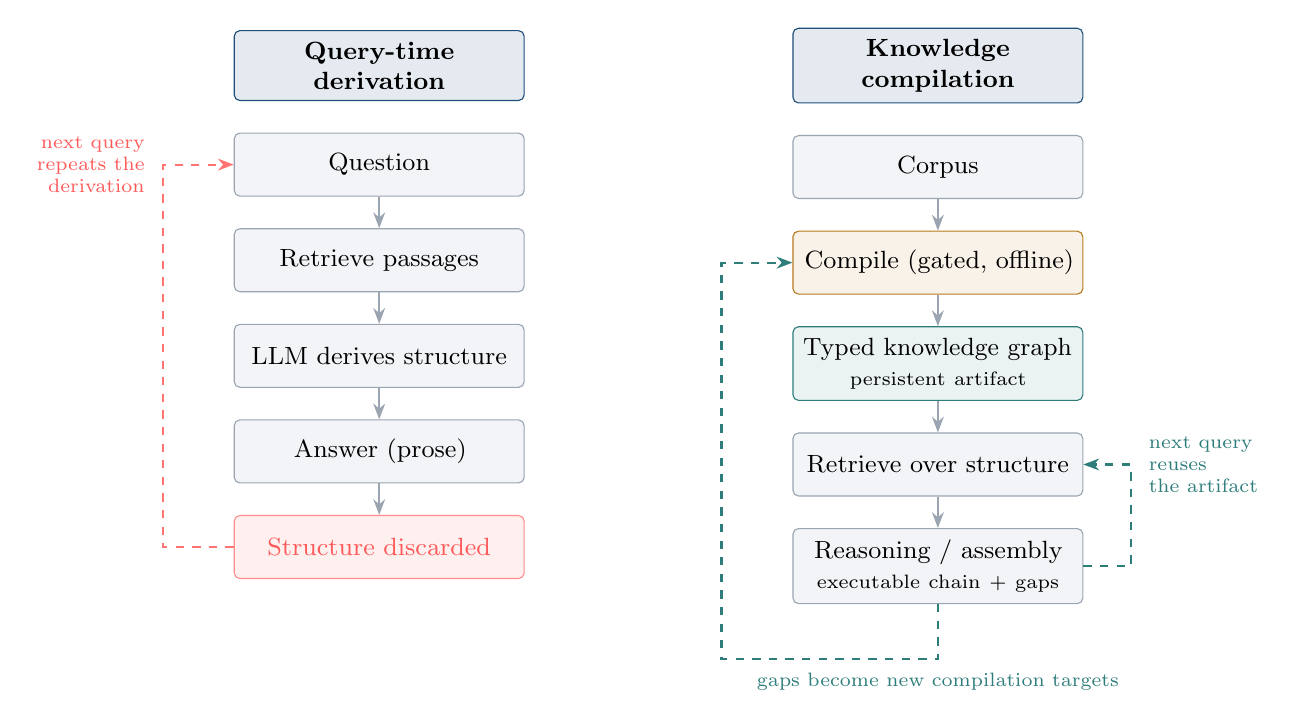
\begin{tikzpicture}[node distance=4mm]
% --- left: query-time
\node[hdr,text width=34mm] (qa) {\textsc{Query-time derivation}};
\node[block,text width=34mm,below=of qa] (q1) {Question};
\node[block,text width=34mm,below=of q1] (q2) {Retrieve passages};
\node[block,text width=34mm,below=of q2] (q3) {LLM derives structure};
\node[block,text width=34mm,below=of q3] (q4) {Answer (prose)};
\node[block,text width=34mm,below=of q4,fill=red!6,draw=red!45] (q5) {\textcolor{red!65}{Structure discarded}};
\draw[ar] (q1)--(q2); \draw[ar] (q2)--(q3); \draw[ar] (q3)--(q4); \draw[ar] (q4)--(q5);
\draw[ar,dashed,draw=red!55] (q5.west) -- ++(-9mm,0) |- (q1.west)
   node[pos=0.5,left,font=\scriptsize,text=red!65,align=right,xshift=-1mm]{next query\\repeats the\\derivation};

% --- right: compiler
\node[hdr,text width=34mm,right=34mm of qa] (ca) {\textsc{Knowledge compilation}};
\node[block,text width=34mm,below=of ca] (c1) {Corpus};
\node[gate,text width=34mm,below=of c1] (c2) {Compile \textnormal{(gated, offline)}};
\node[store,text width=34mm,below=of c2] (c3) {Typed knowledge graph\\{\scriptsize persistent artifact}};
\node[block,text width=34mm,below=of c3] (c4) {Retrieve over structure};
\node[block,text width=34mm,below=of c4] (c5) {Reasoning / assembly\\{\scriptsize executable chain $+$ gaps}};
\draw[ar] (c1)--(c2); \draw[ar] (c2)--(c3); \draw[ar] (c3)--(c4); \draw[ar] (c4)--(c5);
\draw[ar,dashed,draw=ebteal] (c5.east) -- ++(6mm,0) |- (c4.east)
   node[pos=0.5,right,font=\scriptsize,text=ebteal,align=left,xshift=1mm]{next query\\reuses\\the artifact};
\coordinate (gbot) at ($(c5.south)+(0,-7mm)$);
\draw[ar,dashed,draw=ebteal] (c5.south) -- (gbot) -| ($(c2.west)+(-9mm,0)$) -- (c2.west);
\node[font=\scriptsize,text=ebteal,anchor=north] at ($(gbot)+(0,-0.5mm)$)
   {gaps become new compilation targets};
\end{tikzpicture}
\caption{The structural difference. A query-time system performs the expensive
analysis inside the request and discards it; a compiler performs it once and
serves the result. Slogan form: \emph{traditional retrieval compiles on every
query; a knowledge compiler compiles once.}}
\label{fig:why}
\end{figure}

\subsection{What follows from this, and what does not}

Three consequences follow directly, and we state them as claims we can defend:

\begin{enumerate}[leftmargin=1.4em,itemsep=3pt]
\item \textbf{Redundant derivation is eliminated, and the saving grows with
  corpus size.} If $n$ distinct queries or topics all depend on the same
  underlying analysis, a query-time system performs it $n$ times; a compiler
  performs it once. \S\ref{sec:amort} measures $n$ on the live artifact.
\item \textbf{The output is consumable by programs, not only by readers.} A
  passage cannot be type-checked, composed or executed. A typed capability with
  declared inputs, outputs and implementations can be. This is what makes chain
  assembly with explicit gap annotation possible at all
  (\S\ref{sec:runtime}); no amount of retrieval quality produces it.
\item \textbf{Consistency becomes enforceable.} Query-time derivation has no
  global identity: the same capability can be described differently on two
  consecutive queries, and nothing detects it. A compiler has a registry, so
  identity, deduplication and cross-topic linkage are decidable properties
  rather than emergent ones.
\end{enumerate}

We are equally explicit about what does \emph{not} follow. We do \textbf{not}
claim that compilation yields higher answer accuracy than a strong RAG or
GraphRAG baseline, or lower hallucination rates, or better latency. Those are
empirical questions, they require a benchmark that does not currently exist for
robotics engineering knowledge, and we have not run them
(\S\ref{sec:limits}). Nor is compilation free: it moves cost from query time to
build time, and that cost is only worth paying when the same knowledge is
consulted repeatedly --- which is precisely the condition
\S\ref{sec:amort} tests.

\paragraph{Relation to adjacent systems.} The distinction is about \emph{where
the structure lives}, not about which components are used. GraphRAG builds a
graph, but derives it from and for a specific corpus, typically rebuilding
rather than maintaining it, and its nodes are text-derived entities rather than
typed engineering objects with declared interfaces. Agent frameworks and tool
protocols such as MCP standardize \emph{access} to knowledge; they say nothing
about whether the knowledge behind the interface is structured or persistent ---
in fact a compiler is a natural thing to put behind such an interface, and we do
(\S\ref{sec:runtime}). Deep-research products perform excellent query-time
synthesis and discard it. None of these are competitors to compilation; they are
consumers of, or complements to, the artifact it produces.

\subsection{Measuring amortization}
\label{sec:amort}

The claim ``compile once'' is only meaningful if knowledge is in fact reused. We
measure this directly. Let $C$ be the set of distinct compiled capabilities and
$U$ the set of (capability, topic) usages. A query-time system that derived
structure per topic would perform $|U|$ derivations; the compiler performs
$|C|$. We call
\[
\alpha \;=\; \frac{|U|}{|C|}
\]
the \textbf{amortization factor}: the average number of times each compiled unit
is consumed.

On the live artifact, $|C| = 22{,}777$ and $|U| = 36{,}713$, giving
$\alpha = 1.61$. In absolute terms, \textbf{13{,}936 re-derivations are avoided}.
The distribution is heavy-tailed: 6{,}533 capabilities (28.6\%) are used by more
than one topic, and the most reused unit --- \emph{PDDL Problem Instance
Generation} --- is consumed by 32 distinct topics, meaning a query-time system
would re-derive it 32 times.

\begin{figure}[htbp]
\centering
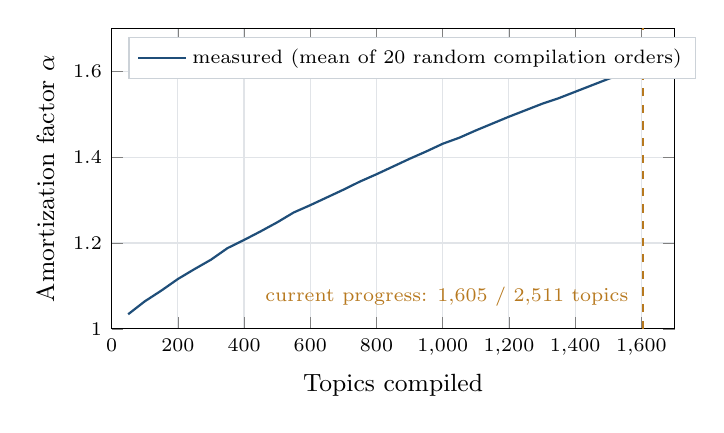
\begin{tikzpicture}
\begin{axis}[
  width=0.72\textwidth, height=5.4cm,
  xlabel={Topics compiled}, ylabel={Amortization factor $\alpha$},
  xmin=0, xmax=1700, ymin=1.0, ymax=1.70,
  grid=major, grid style={draw=ebline!30},
  tick label style={font=\scriptsize}, label style={font=\small},
  legend style={font=\scriptsize, at={(0.03,0.97)}, anchor=north west, draw=ebline!50},
]
\addplot[color=ebblue, thick, mark=none] coordinates {
(50,1.034) (100,1.064) (150,1.089) (200,1.116) (250,1.139) (300,1.161) (350,1.188)
(400,1.207) (450,1.227) (500,1.248) (550,1.271) (600,1.288) (650,1.306) (700,1.324)
(750,1.343) (800,1.360) (850,1.378) (900,1.396) (950,1.413) (1000,1.431) (1050,1.445)
(1100,1.462) (1150,1.478) (1200,1.494) (1250,1.509) (1300,1.524) (1350,1.537)
(1400,1.552) (1450,1.567) (1500,1.582) (1550,1.596) (1600,1.610) (1605,1.612)};
\addlegendentry{measured (mean of 20 random compilation orders)}
\addplot[color=ebamber, dashed, thick, mark=none, forget plot] coordinates {(1605,1.0) (1605,1.70)};
\node[font=\scriptsize, text=ebamber, anchor=south east] at (axis cs:1590,1.03) {current progress: 1{,}605 / 2{,}511 topics};
\end{axis}
\end{tikzpicture}
\caption{Amortization factor as a function of how much of the corpus has been
compiled, averaged over 20 random compilation orders (variance across orders is
negligible at this scale). The curve is still rising at
$+0.029$ per 100 topics in its final quarter and shows no sign of saturation:
the marginal value of compiling one more topic is currently \emph{increasing},
because each new topic is more likely to reuse existing capabilities than to
mint fresh ones. Roughly 36\% of the corpus remains uncompiled.}
\label{fig:amort}
\end{figure}

Figure~\ref{fig:amort} shows the more informative result. Amortization is not a
constant of the system --- it is a function of coverage. At 50 compiled topics
$\alpha \approx 1.03$ (almost nothing is shared yet); at 1{,}605 topics
$\alpha = 1.61$, and the curve has not flattened. This is the property that makes
compilation a sensible investment rather than a one-off cost: the artifact
becomes a better deal the more of the domain it covers, because a capability
minted for one topic is available to every topic compiled afterwards.

\paragraph{Scope of this measurement.} We are measuring \emph{structural} reuse
within our own compilation process --- how often a compiled unit is referenced by
more than one topic. This is a lower bound on, and not the same as, the
derivation savings a deployed query-time system would incur, which depend on
query distribution. It also does not speak to answer quality. We report it
because it is the quantity the ``compile once'' claim is actually about, and
because it is measurable without a benchmark; we do not stretch it further than
that.

% ============================================================
\section{Related Work}
\label{sec:related}

\paragraph{Robot knowledge bases.}
The idea that robots should share structured knowledge has a long lineage.
KnowRob~\cite{tenorth2013knowrob} pioneered a description-logic knowledge
processing system tying symbolic action descriptions to perception and control,
and CRAM~\cite{beetz2010cram} showed how such knowledge drives executable plans.
RoboEarth~\cite{waibel2011roboearth} proposed a shared web database of action
recipes, object models and maps. RoboBrain~\cite{saxena2014robobrain} aggregated
multimodal robotics knowledge into a large graph. IEEE
1872-2015~\cite{ieee1872} standardized a core ontology for robotics and
automation. \eb\ differs from all of these in \emph{what it compiles from} and
\emph{what it compiles to}: prior systems largely encode hand-authored ontologies
or execution traces, whereas \eb\ compiles the open engineering literature and
open-source ecosystem into an engineering-decision graph (which paradigms exist,
what each needs, what implements it) rather than an execution-semantics ontology.
The two are complementary: an engineering-decision graph tells you \emph{which}
grasp planner to use; an execution ontology tells the robot \emph{how} to run it.

\paragraph{Scientific and open knowledge graphs.}
Wikidata~\cite{vrandecic2014wikidata} and DBpedia~\cite{auer2007dbpedia}
demonstrated large-scale collaborative and extracted knowledge graphs; the Open
Research Knowledge Graph~\cite{jaradeh2019orkg} argued for structured, machine-
actionable representations of scholarly contributions. \eb\ shares ORKG's premise
that papers should become structured records, but targets a single vertical
(robotics/embodied AI) at much finer granularity: not ``this paper reports result
$R$'' but ``this paradigm requires these inputs, produces these outputs, fails
under these constraints, and is implemented by these repositories.''

\paragraph{Retrieval.}
Our runtime builds on standard IR components: BM25~\cite{robertson2009bm25},
dense passage retrieval~\cite{karpukhin2020dpr}, cross-encoder
reranking~\cite{nogueira2019passage} and reciprocal rank
fusion~\cite{cormack2009rrf}, with Qwen3-Embedding~\cite{qwen3embedding} as the
encoder. Our contribution here is not a new retrieval algorithm but the
observation that retrieval over a \emph{compiled, typed} corpus admits
structure-aware refinements --- per-facet semantic views with intent-conditioned
weighting, and graph expansion along typed edges --- that are unavailable when
retrieving over raw text.

\paragraph{Multi-agent orchestration and context engineering.}
Decomposing a task across multiple LLM agents is now routine, and the usual
justification is capability specialization --- give each agent the role it is
best at. Our experience (\S\ref{sec:history}) points at a different and, we
think, more binding constraint: the decisive question is not what each agent is
good at but \emph{what can survive the handoff between them}. Our second
architecture failed precisely because it decomposed along role boundaries, and
roles turned out to be the wrong seam --- the seam that mattered was whether the
inter-stage payload was an artifact or a line of reasoning. We are not aware of
this being stated as a design rule, and we offer it as one
(\S\ref{sec:principle}). Relatedly, we treat agent context as a budget to be
allocated by the orchestrator rather than as an accumulating log, and agent
liveness as a systems concern with heartbeats and enforced timeouts
(\S\ref{sec:liveness}) rather than as an exception path.

\paragraph{LLM-based knowledge extraction.}
Using LLMs to construct knowledge graphs is now common practice. The recurring
failure mode is quality: fluent output that is structurally invalid or globally
inconsistent. Our position is that the interesting engineering is not the
extraction prompt but the \emph{admission control and provenance discipline}
around it --- which is why \S\ref{sec:compile} devotes most of its length to
gates and evidence ledgers rather than to generation. The closest analogue we are
aware of is systematic-review methodology in evidence-based medicine, where
recording the search strategy, the databases queried and the studies excluded
with reasons is what separates a review from an opinion. We adopt the same
discipline for machine-generated knowledge, for the same reason.

% ============================================================
\section{System Architecture}
\label{sec:arch}

\eb\ is organized as a strict left-to-right pipeline from raw sources to robot,
with a persistent compiled artifact in the middle
(Figure~\ref{fig:arch}). Everything to the left of the artifact runs offline, in
batch, and is allowed to be slow and expensive. Everything to the right runs
online and consumes the artifact without re-deriving it.

\begin{figure}[htbp]
\centering
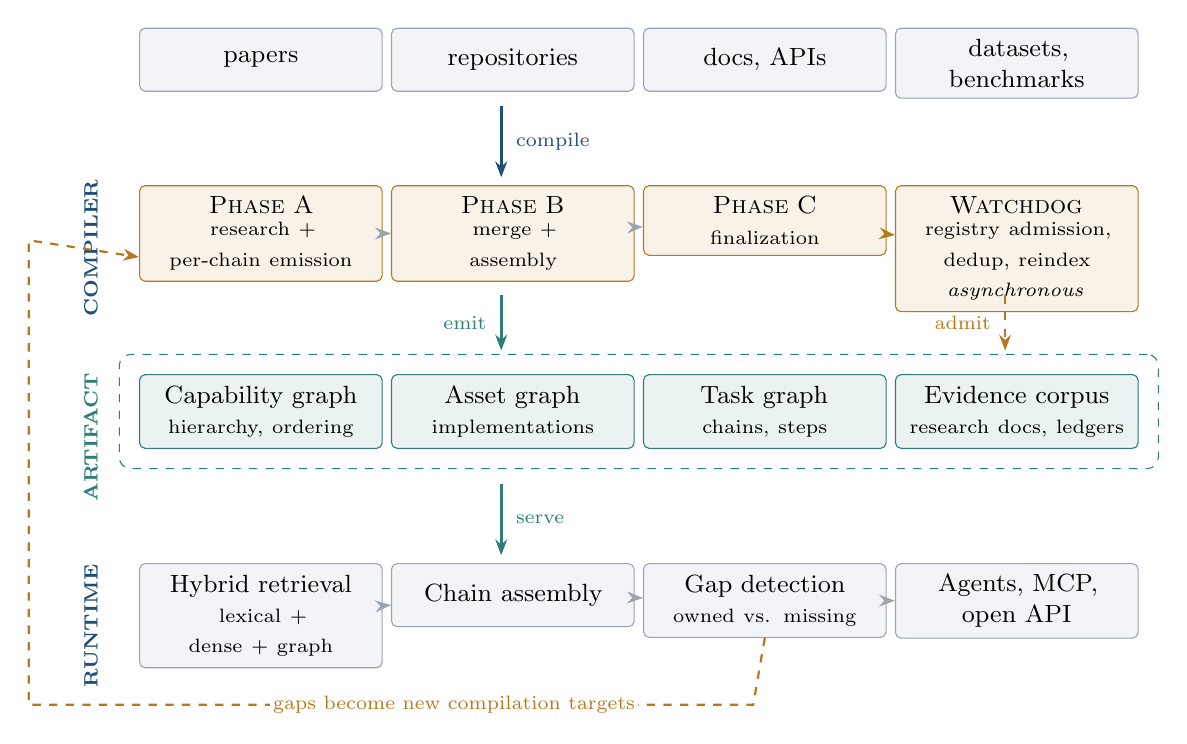
\begin{tikzpicture}[x=1mm,y=1mm]

% ---------- band 1: sources ----------
\node[block,text width=28mm,anchor=north west] (s0) at ( 0,0) {papers};
\node[block,text width=28mm,anchor=north west] (s1) at (32,0) {repositories};
\node[block,text width=28mm,anchor=north west] (s2) at (64,0) {docs, APIs};
\node[block,text width=28mm,anchor=north west] (s3) at (96,0) {datasets,\\benchmarks};

% ---------- band 2: compiler ----------
\node[gate,text width=28mm,anchor=north west] (pA) at ( 0,-20)
   {\textsc{Phase A}\\{\scriptsize research $+$\\per-chain emission}};
\node[gate,text width=28mm,anchor=north west] (pB) at (32,-20)
   {\textsc{Phase B}\\{\scriptsize merge $+$\\assembly}};
\node[gate,text width=28mm,anchor=north west] (pC) at (64,-20)
   {\textsc{Phase C}\\{\scriptsize finalization}};
\node[block,text width=28mm,anchor=north west,fill=ebamber!10,draw=ebamber] (wd) at (96,-20)
   {\textsc{Watchdog}\\{\scriptsize registry admission,\\dedup, reindex}\\{\scriptsize\emph{asynchronous}}};
\draw[ar] (pA)--(pB);
\draw[ar] (pB)--(pC);
\draw[ar,dashed,draw=ebamber] (pC)--(wd);

% ---------- band 3: artifact ----------
\node[store,text width=28mm,anchor=north west] (g0) at ( 0,-44)
   {Capability graph\\{\scriptsize hierarchy, ordering}};
\node[store,text width=28mm,anchor=north west] (g1) at (32,-44)
   {Asset graph\\{\scriptsize implementations}};
\node[store,text width=28mm,anchor=north west] (g2) at (64,-44)
   {Task graph\\{\scriptsize chains, steps}};
\node[store,text width=28mm,anchor=north west] (g3) at (96,-44)
   {Evidence corpus\\{\scriptsize research docs, ledgers}};

% ---------- band 4: runtime ----------
\node[block,text width=28mm,anchor=north west] (r0) at ( 0,-68)
   {Hybrid retrieval\\{\scriptsize lexical $+$ dense $+$ graph}};
\node[block,text width=28mm,anchor=north west] (r1) at (32,-68)
   {Chain assembly};
\node[block,text width=28mm,anchor=north west] (r2) at (64,-68)
   {Gap detection\\{\scriptsize owned vs. missing}};
\node[block,text width=28mm,anchor=north west] (r3) at (96,-68)
   {Agents, MCP,\\open API};
\draw[ar] (r0)--(r1); \draw[ar] (r1)--(r2); \draw[ar] (r2)--(r3);

% ---------- artifact enclosure (drawn before vertical arrows) ----------
\begin{scope}[on background layer]
\node[draw=ebteal,dashed,rounded corners,fit=(g0)(g3),inner sep=2.5mm] (artbox) {};
\end{scope}

% ---------- vertical band-to-band flows ----------
\draw[ar,very thick,draw=ebblue] (46,-10) -- (46,-19)
      node[midway,right=0.5mm,font=\scriptsize,text=ebblue]{compile};
\draw[ar,very thick,draw=ebteal] (46,-34) -- (46,-41)
      node[midway,left=0.5mm,font=\scriptsize,text=ebteal]{emit};
% watchdog admits registry entities into the artifact
\draw[ar,dashed,thick,draw=ebamber] (110,-34) -- (110,-41)
      node[midway,left=0.5mm,font=\scriptsize,text=ebamber]{admit};
\draw[ar,very thick,draw=ebteal] (46,-58) -- (46,-67)
      node[midway,right=0.5mm,font=\scriptsize,text=ebteal]{serve};

% ---------- band labels ----------
\node[font=\scriptsize\bfseries,text=ebblue,rotate=90,anchor=south] at (-4,-28) {COMPILER};
\node[font=\scriptsize\bfseries,text=ebteal,rotate=90,anchor=south] at (-4,-52) {ARTIFACT};
\node[font=\scriptsize\bfseries,text=ebblue,rotate=90,anchor=south] at (-4,-76) {RUNTIME};

% ---------- feedback: gap detection -> phase A ----------
\draw[ar,dashed,thick,draw=ebamber]
   (r2.south) -- (78,-86) -- (-14,-86) -- (-14,-27) -- ($(pA.west)+(0,-3)$);
\node[font=\scriptsize,text=ebamber,fill=white,inner sep=1pt] at (40,-86)
   {gaps become new compilation targets};
\end{tikzpicture}
\caption{\eb\ end to end. The compiled artifact (dashed box) is the durable
product: everything above it is an offline batch compiler, everything below it is
a consumer. Registry admission and index maintenance run asynchronously in a
separate watchdog, outside the compilation transaction (\S\ref{sec:watchdog}).
Gaps found at runtime return as new compilation targets.}
\label{fig:arch}
\end{figure}

\subsection{The taxonomy backbone}

Compilation is not undirected crawling. It is driven by a manually curated
three-level taxonomy that defines \emph{what should exist}, so that coverage is
measurable and boundaries between topics are explicit. The current tree has
2{,}942 nodes:

\begin{center}
\small
\begin{tabular}{@{}llr@{}}
\toprule
Level & Meaning & Count \\
\midrule
L0 & Top-level domain & 15 \\
L1 & Sub-domain & 416 \\
L2 & Compilation unit (topic) & 2{,}511 \\
\midrule
& Total & 2{,}942 \\
\bottomrule
\end{tabular}
\end{center}

\noindent The 15 L0 domains are: Foundation Models, Human-Robot Interaction,
Learning, Localization, Manipulation, Mapping, Motion \& Control, Multi-Robot
Systems, Navigation, Perception, Planning, Reasoning \& Agent, Safety/Trust \&
Security, Simulation \& Digital Twin, and System Infrastructure.

The L2 node is the \textbf{unit of compilation}: one L2 topic (for example
\texttt{a\_star\_path\_}\allowbreak\texttt{planning} or
\texttt{finger\_gait\_planning}) is compiled in
one transaction, producing one topic record containing several task chains and
the capabilities and assets they reference. Sibling L2 nodes are passed to the
extractor as explicit \emph{boundary constraints}, which is how the system
prevents adjacent topics from absorbing each other's content --- the compiler's
equivalent of scoping rules.

% ============================================================
\section{Knowledge Compilation}
\label{sec:compile}

This section describes the compiler. We lead with its architectural history,
because the current design is the third attempt and the two failures are more
instructive than the survivor.

\subsection{Two failed architectures}
\label{sec:history}

\paragraph{v1 --- one agent, one topic, one context.} The original compiler gave
a single agent the whole topic: research everything, then write the whole record.
It failed in three ways that turned out to be the same failure. Research depth
was squeezed by context length --- as the conversation filled with retrieved
material, later chains got shallower treatment than earlier ones. Information
from different technical paradigms contaminated each other, so chains converged
toward a common vocabulary that belonged to none of them. And by the time the
agent wrote the record, a large fraction of fields were \emph{drafted from
memory} rather than grounded in anything retrieved; the research documents
degenerated into conclusions with no recoverable evidence behind them.

\paragraph{v2 --- one agent per chain, split into a relay.} The obvious fix was
to give each technical chain its own context. We did that, and further split each
chain across three specialist agents in sequence --- research, then asset
verification, then JSON emission --- with all chains completing research before
any chain entered generation. This version failed for a reason we did not
anticipate and now consider the most important lesson in the project:

\begin{quote}
\textbf{Design intent evaporates at the handoff.} Why this chain has \emph{this}
step sequence; why step 4 must follow step 3; why two capabilities were not
split apart --- these are judgments formed \emph{during} research. Only their
conclusions can be written into a document. The reasoning that produced them
cannot.
\end{quote}

\noindent The downstream agent therefore had no choice but to transcribe the
document literally. Two consequences followed. First, when the document did not
cover a field, the JSON agent had no recourse: it was forbidden from searching
(without research context, a searching agent fabricates from memory), so a gap
that one query would have closed had to wait for human intervention or an entire
additional session. Second, the asset-verification agent could not feed back: on
discovering that a capability had no real implementation anywhere, it had neither
the authority nor the context to revise the capability list the research agent
had designed. It could only execute.

\subsection{The principle: split on artifacts, merge on reasoning}
\label{sec:principle}

The resolution generalizes beyond this system, and it is the design rule we
would most want a reader to take away:

\begin{quote}
\textbf{Merge two stages into one context when what passes between them is
reasoning. Split them into separate contexts when what passes between them is an
artifact.}
\end{quote}

\noindent Reasoning does not survive serialization; artifacts do. A handoff that
requires the receiver to reconstruct \emph{why} is a handoff that should not
exist. A handoff that requires the receiver only to consume \emph{what} is a
handoff that should be made explicit, durable and resumable.

Applied to this compiler, the rule cuts in two directions at once, which is why
the resulting architecture looks inconsistent until the rule is stated:

\begin{itemize}[leftmargin=1.4em,itemsep=2pt]
\item \textbf{Within a chain, merge.} Research, asset verification and record
  emission happen in \emph{one} agent session, because what passes between them
  is design intent.
\item \textbf{Across the orchestration, split.} Panoramic scan, cross-chain
  merge, and final validation happen in \emph{three separate} agent sessions
  handing off through the file system, because what passes between them is
  finished artifacts --- documents, fragments, a record.
\end{itemize}

\subsection{v3: chain-level closed loop under a three-phase orchestrator}

Figure~\ref{fig:pipeline} shows the resulting architecture.

\begin{figure}[htbp]
\centering
\begin{tikzpicture}[x=1mm,y=1mm]

% column x-origins
\def\ca{0}\def\cb{55}\def\cc{110}
\def\cw{46}

% ---------- headers ----------
\node[hdr,text width=\cw mm,anchor=north west] (hA) at (\ca,0)
  {\textsc{Phase A}\\{\scriptsize research $+$ per-chain emission}};
\node[hdr,text width=\cw mm,anchor=north west] (hB) at (\cb,0)
  {\textsc{Phase B}\\{\scriptsize merge $+$ assembly}};
\node[hdr,text width=\cw mm,anchor=north west] (hC) at (\cc,0)
  {\textsc{Phase C}\\{\scriptsize finalization}};

\draw[ar,very thick,draw=ebteal] (hA.east) -- (hB.west)
   node[midway,above,font=\scriptsize,text=ebteal]{disk};
\draw[ar,very thick,draw=ebteal] (hB.east) -- (hC.west)
   node[midway,above,font=\scriptsize,text=ebteal]{disk};

% ---------- column A ----------
\node[block,text width=\cw mm,anchor=north west] (a1) at (\ca,-18)
  {Panoramic scan\\{\scriptsize candidate chain list}};
\node[gate,text width=\cw mm,anchor=north west] (a2) at (\ca,-33)
  {\textbf{Red-team review}\\{\scriptsize fresh context: omissions, errors,\\granularity, ordering}};
\node[block,text width=\cw mm,anchor=north west] (a3) at (\ca,-53)
  {Dispatch one closed-loop\\agent \emph{per chain}\\{\scriptsize anchoring card $=$ boundary}};
\node[gate,text width=\cw mm,anchor=north west] (a4) at (\ca,-73)
  {Chain quality gate\\{\scriptsize 5 criteria; pass / void / manual;\\${\geq}2$ chains must pass}};
\draw[ar] (a1)--(a2); \draw[ar] (a2)--(a3); \draw[ar] (a3)--(a4);

% ---------- column B ----------
\node[block,text width=\cw mm,anchor=north west] (b1) at (\cb,-18)
  {Entity-level identifier\\normalization};
\node[block,text width=\cw mm,anchor=north west] (b2) at (\cb,-33)
  {Chain overlap adjudication\\{\scriptsize $|A\cap B| / \min(|A|,|B|)$}};
\node[block,text width=\cw mm,anchor=north west] (b3) at (\cb,-50)
  {Assemble topic record};
\node[block,text width=\cw mm,anchor=north west] (b4) at (\cb,-62)
  {\emph{Then} rekey to surrogate\\identifiers\\{\scriptsize order matters --- \S\ref{sec:order}}};
\draw[ar] (b1)--(b2); \draw[ar] (b2)--(b3); \draw[ar] (b3)--(b4);

% ---------- column C ----------
\node[gate,text width=\cw mm,anchor=north west] (c1) at (\cc,-18)
  {Script gates\\{\scriptsize structural validation,\\finalization check, conflict check}};
\node[block,text width=\cw mm,anchor=north west] (c2) at (\cc,-38)
  {Single repair\\{\scriptsize no loop; else failure ledger}};
\node[gate,text width=\cw mm,anchor=north west] (c3) at (\cc,-53)
  {Judgment gates\\{\scriptsize synonym warnings, unverified\\fields, paradigm distinctness}};
\node[store,text width=\cw mm,anchor=north west] (c4) at (\cc,-73)
  {Topic record on disk};
\draw[ar] (c1)--(c2); \draw[ar] (c2)--(c3); \draw[ar] (c3)--(c4);

% ---------- watchdog ----------
\node[block,text width=\cw mm,anchor=north west,fill=ebamber!10,draw=ebamber] (wd) at (\cb,-88)
  {\textsc{Watchdog} \emph{(asynchronous)}\\{\scriptsize registry write, duplicate\\adjudication, vector reindex}};
\draw[ar,dashed,thick,draw=ebamber] (c4.south) -- ++(0,-6) -| (wd.east);
\node[font=\scriptsize,text=ebamber,anchor=north] at ($(wd.south)+(0,-2)$)
  {\emph{No agent in phases A--C may write the registry or the index.}};
\end{tikzpicture}
\caption{The three-phase compilation architecture. Phases hand off through the
file system and share no conversation context; within phase A, each chain is
compiled by a single closed-loop agent. Registry writes and index maintenance are
performed asynchronously by a separate watchdog and are explicitly outside the
compilation transaction.}
\label{fig:pipeline}
\end{figure}

\paragraph{The chain-level closed loop.} One agent owns one chain end to end:
segment A researches the chain's structure, segment B verifies its assets,
segment C emits the JSON fragment --- all in one session, then the session exits
and its context is released. Because the agent that writes the record is the
agent that did the research, gaps discovered during emission can be closed by a
few additional queries on the spot, and segment B can revise decisions made in
segment A. The agent reads one specification file per segment rather than loading
all three up front, since pre-loading would spend the context the closed loop was
meant to save.

The cost of this design is that chains run in parallel and mint identifiers
independently, so the same real capability reliably acquires two identifiers
under two names. That cost is paid, deliberately and in one place, by Phase B.
The trade is favourable because \emph{merging is mechanically decidable} --- it
has criteria, thresholds and a written adjudication standard --- whereas design
intent, once lost, cannot be reconstructed at any price.

A secondary benefit is scheduling: agents per topic fall from $3N$ to $N$. A
five-chain topic went from fifteen dispatch/recover cycles to five, reducing both
orchestration overhead and the number of opportunities for a node to hang.

\paragraph{Why the orchestrator still splits into three.} The closed loop solves
context pressure for a chain but not for the controller, which would otherwise
accumulate breakpoint inventory, service checks, the panoramic scan, $N$ rounds
of dispatch and recovery, per-chain gating, cross-chain merge adjudication,
assembly, rekeying and final validation in one context. Crowding would be worst
exactly at merge and final validation --- the two stages that most need cold
judgment. Splitting is possible only because resumability already required every
intermediate product to be identifiable and reusable on disk; the phase boundary
is an existing internal breakpoint promoted to an inter-agent handoff.

\subsection{Phase A: research and per-chain emission}
\label{sec:phaseA}

\paragraph{Boundary contract.} Every dispatched agent receives, verbatim and
inside its fence, the topic's \emph{anchoring card}: the scope statement, the
sibling-topic list and the explicit exclusions. Paraphrasing it or referring to
it by path is forbidden. This is the mechanism that stops adjacent topics from
absorbing each other's content; a chain agent that finds material belonging to a
sibling records a cross-reference rather than expanding into it.

\paragraph{Red-team review.} After the panoramic scan produces a candidate chain
list, that list is submitted to a \emph{fresh conversation} for adversarial
review against four questions: what important technical routes are missing; which
chains have mis-assigned paradigms, wrong representative systems or wrong
citations; whether any chain's granularity is too coarse or too fine; and whether
the ordering is defensible. The conclusions are written into the research
document and the candidate list is revised before any chain is dispatched.

Two properties make this worth its cost. It runs in a clean context, so it is not
anchored by the reasoning that produced the list. And it runs at the cheapest
possible moment: merging two near-duplicate candidate chains here costs one
edit, whereas discovering the duplication after both have run full closed-loop
compilation costs two wasted agent sessions and a merge adjudication.

\paragraph{Evidence floors and the retrieval ledger.} Within a chain agent,
segment A must perform at least 10 web searches and 8 page fetches, and segment B
at least 6 and 8 respectively, plus registry lookups and repository verification
calls. Every one is logged. \S\ref{sec:evidence} describes the ledger format,
including its mandatory negative-results table.

\paragraph{Context-budget discipline.} When a chain agent returns, the controller
records \emph{one line} --- chain number, verdict, entity counts, whether gaps
were flagged --- and does not read the returned artifacts into its own context.
This is explicit in the specification: the controller's context is reserved for
dispatch and gating decisions. Treating context as a budget to be allocated,
rather than as a place where information accumulates, is what makes a 30-topic
batch tractable.

\paragraph{Recovery gates and non-binary verdicts.} Each returned chain is
validated twice by script --- once for the research document, once for the
fragment --- and both must report zero errors. The controller then applies a
five-criterion quality rubric (Table~\ref{tab:chaingate}). Verdicts are
deliberately \emph{not} binary: a chain may pass, be voided, or be marked
\emph{manual intervention} after two failed reruns. Voided chains keep their
fragments on disk for the record but are marked ``not to be assembled''. A
chain that cannot be settled does not block the batch.

\begin{table}[htbp]
\centering\small
\caption{Phase-A single-chain quality rubric. Note that ``negative evidence''
--- routes and assets that were investigated and rejected --- is a graded
criterion, not an optional courtesy.}
\label{tab:chaingate}
\begin{tabular}{@{}p{38mm}p{62mm}p{34mm}@{}}
\toprule
Criterion & Pass condition & On failure \\
\midrule
Real-system support & chain maps to an identifiable engineering system or paper & void the chain \\
Step sufficiency & ${\geq}4$ sub-steps (phase nodes do not count) & redispatch or void \\
Dataflow coherence & each step's inputs connect to prior outputs; no magic steps & redispatch \\
Derivation completeness & the five design questions are all answered and coherent & redispatch \\
Negative evidence & investigated-but-rejected routes and assets are recorded & warning only \\
\bottomrule
\end{tabular}
\end{table}

\noindent If fewer than two chains pass, the controller returns to the panoramic
scan rather than lowering the bar --- a topic with one paradigm is a signal that
the scan was incomplete, not that the topic is simple.

\paragraph{Findings, not decisions.} Phase A closes with a cross-chain registry
spot-check: does the same real project resolve to the same registry identifier in
every chain that used it? Discrepancies are recorded as \emph{leads for Phase B}
and explicitly not acted upon, because a controller that starts merging here
would collide with the phase that owns merging.

\subsection{Phase B: merge and assembly}
\label{sec:phaseB}

Phase B is the only point in the entire flow with simultaneous visibility of
every finished chain, and it does its own work rather than delegating --- the
judgment required is exactly what would be lost by dispatching it. It is
correspondingly the phase we allocate the strongest available model to.

\paragraph{Entity-level normalization.} Every cross-chain pair of similar
entities is adjudicated same/different under a written standard shared with the
global deduplication process. Assets carry a hard rule: two assets whose sources
are different repositories are different, however similar their descriptions, and
independently installable sub-packages of a monorepo are distinct assets. When
merging, the surviving identifier is the one already present in the global
registry if either is; the discarded entity's unique applicability and constraint
text is folded into the survivor before the merge, not after. Uncertain pairs are
left unmerged, on the standing argument that a false merge destroys a distinction
irreversibly while a false retention is corrected later at no loss.

\paragraph{Chain overlap adjudication.} With identifiers normalized, pairwise
chain overlap is computed over capability sets only:
\[
\mathrm{overlap}(A,B) \;=\; \frac{|A \cap B|}{\min(|A|,|B|)} .
\]
Assets are excluded deliberately --- two chains both using PyTorch are not the
same chain. Overlap ${\geq}0.70$ merges the pair; $[0.50, 0.70)$ is a grey band
requiring the adjudicator to read both chains' research documents and decide on
the basis of whether they target the same real system or family; below $0.50$
both are kept. Merged chains inherit a provenance sentence recording which chains
were combined, at what overlap, and under which criterion --- and, importantly,
\emph{both} original research documents remain referenced by the assembled
record, because dropping one would delete that paradigm's entire research corpus
from the evidence index.

\subsection{Two ordering constraints}
\label{sec:order}

Two sequencing rules in Phase B are, in our view, the most transferable technical
findings in the system. Both are cases where a locally reasonable order silently
degrades a decision made later.

\paragraph{Normalize entities before measuring chain overlap.} If the same
capability still carries two identifiers in two chains, it counts as
non-overlapping, and the overlap ratio is systematically \emph{under}-estimated
--- precisely for the chain pairs that are most redundant, because those are the
pairs with the most shared capabilities and therefore the most duplicate
identifiers. Highly overlapping chains would then never be merged. The bias is
not random noise; it is anticorrelated with the thing being measured.

\paragraph{Rekey identifiers after merging, never before.} Capability
identifiers are opaque surrogate keys (\S\ref{sec:g2}), which is the right
representation for storage. But the merge decision is a semantic judgment made by
reading names and descriptions. Rekeying first would present the adjudicator with
two hexadecimal strings and no way to see that they denote the same thing; the
specification's own phrasing is that adjudication quality falls off a cliff.

The general lesson is that surrogate keys are not uniformly good. They are
correct for reference and storage and actively harmful in any stage whose input
is human-or-model semantic judgment. A system that uses them must therefore be
explicit about \emph{when} the transition from names to keys occurs --- and it
should occur as late as possible, after every stage that needs to read.

\subsection{Phase C: finalization}
\label{sec:phaseC}

Phase C validates and does not generate. Script gates run first: structural
validation, a finalization checker, and a registry conflict check in
\texttt{-{}-check} mode. The finalization checker deliberately partitions its own
output into \emph{blocking} findings, which it asserts have no false positives
and must be fixed, and \emph{informational} findings, which it acknowledges do
have false positives and are passed to judgment rather than enforced. We regard
this self-classification as good practice: a checker that does not distinguish
what it is certain about from what it is guessing at will eventually be ignored
wholesale.

Repair is dispatched \emph{once}. If the gates still fail, the topic goes to a
failure ledger for human attention rather than into a repair loop.

Phase C also carries an explicit \emph{time-discipline} instruction that we think
is underappreciated in agent system design: it is forbidden to re-read the chain
research documents in full, to re-verify asset URLs, or to redo the adversarial
reading already performed upstream. The stated reason is that the acceptance
records of those earlier steps \emph{are} the evidence, and repeating them
consumes budget without improving quality. Without such an instruction, a
capable agent given a validation role will re-derive everything it can, and a
pipeline that re-validates at every stage does not converge.

One judgment rule from this phase deserves quoting on its own, because it
inverts the usual optimization pressure: where a field could not be verified, the
agent must leave it marked unverified, and \emph{fabricating a citation to make
the unverified-field count go down is treated as a far more serious failure than
leaving the field unverified.}

\subsection{Registry writes are outside the transaction}
\label{sec:watchdog}

No agent in Phases A--C may write the global registry or the vector index. The
orchestrator and all task nodes are prohibited from invoking registry
synchronization other than in check mode, and from any index write. Real registry
admission, duplicate adjudication and index maintenance are performed
asynchronously by a separate watchdog process; the orchestrator's only
post-processing step is a version-control commit.

This is a meaningful correction to the naive picture of a compiler in which
linking is the last stage of each translation unit. Here, per-topic compilation
and global registry admission are decoupled: 30 topics compile concurrently
without contending for the registry, and a registry problem cannot stall
compilation. The cost is that the invariant ``everything in the registry is
structurally valid'' is enforced at admission by the watchdog rather than by the
compiling agent, and that the registry lags the topic records by the watchdog's
period.

\subsection{Liveness, idempotence and failure}
\label{sec:liveness}

Compilation runs unattended and continuously, so the orchestration treats agent
liveness as a first-class systems problem rather than an exception path.

\begin{itemize}[leftmargin=1.4em,itemsep=2pt]
\item \textbf{Heartbeats are file mtimes.} A chain agent appends to its retrieval
  ledger every two to three tool calls. This serves two purposes at once: it
  offloads context, and it produces an observable file-system heartbeat. Three
  minutes without a file change is treated as death.
\item \textbf{Timeouts are tiered and enforced by killing.} Per-node caps are 40,
  20 and 15 minutes for phases A, B and C; a phase round caps at 90 minutes and a
  30-topic batch targets two hours. On timeout the node is killed --- not
  diagnosed, not retried within the round.
\item \textbf{Idempotence is by artifact existence.} A topic whose record exists
  is done and is never touched again, regardless of any status file; status
  metadata is explicitly distrusted in favour of the file system.
\item \textbf{Timed-out work is not failed work.} A killed topic is \emph{not}
  written to the failure ledger. It produced no record, so the next scan returns
  it to the pending set naturally. Only topics that failed validation after
  repair are recorded as failures --- the ledger means ``needs a human'', not
  ``did not finish''.
\item \textbf{Resumption is per-step, not per-topic.} Every phase begins with a
  breakpoint inventory that skips completed steps, so a killed topic resumes
  rather than restarting.
\end{itemize}

\noindent The batch loop follows from these: the pending set is computed as
taxonomy $\cap$ $\neg$disk $\cap$ $\neg$failure-ledger, 30 topics are advanced
through phase A, then B, then C, and the loop repeats without waiting for
stragglers.

\subsection{Allocating model capability}
\label{sec:models}

Because the phases differ in what they demand, model capability is allocated
rather than applied uniformly:

\begin{center}\small
\begin{tabular}{@{}p{40mm}p{56mm}p{40mm}@{}}
\toprule
Role & Dominant demand & Allocation \\
\midrule
Phase B (merge) & cross-document same/different judgment & strongest available \\
Phase A (scan, gating) & domain breadth; the candidate list caps everything downstream & strong \\
Chain closed-loop agent & search planning, evidence discrimination \emph{and} schema compliance & strong; low temperature \\
Red-team review & critical checking; one-shot & inexpensive relative to the rework it prevents \\
Phase C (finalization) & mechanical checking; scripts carry most of the load & mid-tier \\
\bottomrule
\end{tabular}
\end{center}

\paragraph{Two different kinds of model use.} It is worth separating them, since
they are often conflated. \emph{Compilation} is performed by tool-using agents in
an agent harness --- they search the web, fetch pages, run verification scripts,
read and write files, and dispatch sub-agents; the roles above refer to these.
\emph{Runtime and auxiliary services} --- query intent decomposition, gap
detection, chain assembly and duplicate adjudication --- are ordinary API calls to
a separate, cheaper chat model behind a single client abstraction, with
temperature and model selectable per call site (low temperature and a
retention-biased instruction for duplicate adjudication, for instance). The
compiler needs agency; the runtime services need throughput.

\noindent The specification records one explicit warning here: the chain agent
must \emph{not} be downgraded on the reasoning that asset verification is
routine, because the same session goes on to emit the schema-conformant record.
Closing the loop removed the option of using a cheap model for the mechanical
segment --- a real and acknowledged cost of the design.


\subsection{The Retrieval Ledger}
\label{sec:evidence}

Within the chain agent, evidence gathering is where factual grounding is enforced,
and it is the part of the system we consider most consequential.
Segment A is where the system's factual grounding is enforced, and it is the part
we consider most consequential. Every chain research document must terminate in a
mandatory \textbf{retrieval log}. The specification instructs floors of at least 10
web searches and 8 page fetches for the paradigm-research segment and 6 and 8 for
the asset-research segment; the mechanical validator checks that the ledger section
is present and well-formed, but does not itself compare the recorded counts against
those floors, so compliance is instructed rather than enforced. In a random sample
of 400 topic directories, documents carrying a parsable ledger record a median of 10
searches and 6 fetches, and 46\% meet both instructed floors. Enforcing the counts
in the validator is a small change we have not yet made. The log is not a summary count. It has four parts:

\begin{enumerate}[leftmargin=1.4em,itemsep=2pt]
\item a \textbf{per-query table} recording every search issued, its hit count, the
  key systems/papers/terms it surfaced, and \emph{which section of the document
  the result was used in} --- so an unused query is visibly unused;
\item a \textbf{fetch and script table} recording every page fetched and every
  verification script invocation, with the extracted evidence quoted;
\item a \textbf{negative-results table} listing candidates that were found and
  \emph{deliberately excluded}, with the exclusion rationale and the log line the
  candidate came from;
\item a \textbf{registry-lookup record} showing which existing capabilities the
  research reused rather than re-minting.
\end{enumerate}

Repository claims are not taken on the model's word: a verification script
queries each candidate GitHub repository and returns its real star count, license
and README text, which is quoted into the log. A paper-fetch script does the same
for literature. A chain document that cannot ground a claim is required to mark
it explicitly as unverified rather than assert it.

Table~\ref{tab:ledger} reproduces an excerpt of a real ledger. Its most unusual
feature is that it records \emph{failure}: queries that returned nothing useful,
and candidates that were rejected. A generated document that only ever reports
successful retrieval is indistinguishable from a fabricated one; a ledger with
honest negative entries is not.

\begin{table}[htbp]
\centering\small
\caption{Excerpt from the retrieval ledger of a real chain research document
(\texttt{evaluation\_metric\_definition}, chain 01). Translated from the stored
Chinese. Note the recorded failures --- the mechanism's credibility rests on
them.}
\label{tab:ledger}
\begin{tabular}{@{}p{4mm}p{58mm}p{13mm}p{45mm}@{}}
\toprule
\# & Query / action & Used in & Outcome \\
\midrule
\multicolumn{4}{@{}l}{\textit{Search log}}\\
1 & RLBench success\_criteria task.py programmatic success determination PyRep & \S1, \S8 & 5 hits; weak sources \\
2 & RLBench \_success\_criteria TaskStatus method stepjam github & --- & 5 hits; \emph{no direct hit} \\
3 & MetaWorld success flag termination condition manipulation benchmark & --- & 5 hits; \emph{no direct hit} \\
4 & LIBERO benchmark BDDL goal condition success MuJoCo & \S1, \S8 & BDDL format confirmed \\
\midrule
\multicolumn{4}{@{}l}{\textit{Fetch / script log}}\\
1 & \texttt{check\_github.py stepjam/RLBench} & \S1, \S10, \S11 & 1802 stars, License: Other; README quoted verbatim \\
3 & \texttt{check\_github.py Farama-Foundation/Metaworld} & \S1, \S10, \S11 & 1859 stars, MIT; Gymnasium API confirmed \\
4 & \texttt{registry\_lookup.py "RLBench success criteria"} & \S5--\S7 & 23 hits / 8 vector; 10 existing capabilities reused \\
\midrule
\multicolumn{4}{@{}l}{\textit{Negative results (found, then excluded)}}\\
--- & ALFWorld task-level success determination & --- & text-embodied, not simulation manipulation; belongs to sibling topic \\
--- & Real-robot multimodal success detection & --- & no ground truth on real hardware; out of chain scope \\
\bottomrule
\end{tabular}
\end{table}

This regime is being rolled out across the corpus rather than applied
retroactively. In a random sample of 220 topic directories (706 chain documents),
43.6\% carry a full retrieval ledger, and those that do average 9.1 recorded
searches and 6.1 recorded fetches in the paradigm-research segment alone;
225 of the 706 sampled chain documents (31.9\%) carry a negative-results table.
Documents compiled under the earlier regime remain in the artifact and are
scheduled for re-compilation.

The intermediate evidence documents are retained as first-class artifacts, not
discarded scaffolding: the compiler currently holds 5{,}510 chain research
documents across 1{,}698 topic directories, an average of 3.24 chains per
compiled topic. This means every capability in the graph is traceable back to the
document that produced it, and that document to the queries that grounded it.


\subsection{The structural validator}
\label{sec:g1}

A task chain is a directed graph: steps carry \texttt{next} pointers, and
branch/merge steps are permitted. LLM output is fluent but routinely produces
graphs that are subtly illegal --- unreachable steps, cycles, references to
capability identifiers that do not exist. The validator checks this with three classical
graph algorithms:

\begin{enumerate}[leftmargin=1.4em,itemsep=2pt]
\item \textbf{In-degree analysis} to locate entry nodes. A chain with no
  zero-in-degree node is almost always cyclic.
\item \textbf{DFS/BFS reachability} from the entry set. Any unvisited node is
  orphaned and reported.
\item \textbf{Tri-colour marking} (white/grey/black) for strict cycle detection:
  encountering a grey node during traversal is a back edge, hence a cycle.
\end{enumerate}

Beyond graph structure, it enforces roughly twenty additional rules: bidirectional
consistency of capability parent/child declarations (if $p$ lists $c$ as a child,
$c$ must list $p$ as parent), identifier format, asset reference integrity, and a
platform-asset blacklist that forbids attaching generic platforms (ROS, PyTorch)
directly to a specific algorithmic capability --- a rule that exists because
without it the implementation graph degenerates into everything pointing at ROS.
Rules are two-tier: \texttt{ERROR} aborts the compilation unit with a non-zero
exit; \texttt{WARN} is recorded but does not block.


\subsection{Registry admission and global deduplication}
\label{sec:g2}

Because compilation is per-topic and independent, the same capability
(``inverse kinematics solving'') will be independently rediscovered by many
topics. Registry admission is the linker: it decides whether an entity arriving
from a compiled topic record is new, is an existing entity, or is a conflict.
As described in \S\ref{sec:watchdog}, this runs asynchronously in the watchdog;
the compiling agents only ever run it in check mode.

\paragraph{Hard conflicts.} If an identifier is already occupied by an entity of
a different type or a different upstream repository, the entire write is
rejected. There is no partial admission.

\paragraph{Suspect detection --- primary path.} The current primary path is
embedding-based. Each candidate and each incumbent are encoded into two views:
\emph{identity} (name and aliases) and \emph{concept} (description). With
$s_{\text{id}}$ and $s_{\text{con}}$ the respective cosine similarities, the
combined score is
\[
s \;=\; 0.5\,s_{\text{id}} \;+\; 0.5\,s_{\text{con}},
\]
and a pair is flagged as a duplicate suspect when
\[
s \geq 0.86 \quad\text{or}\quad \max(s_{\text{id}}, s_{\text{con}}) \geq 0.95 .
\]
Both thresholds were set empirically against a snapshot of roughly 9{,}099
capability vectors, in which the 95th percentile of \emph{legitimate}
nearest-neighbour similarity was $\approx 0.863$: the threshold sits at the
background noise ceiling rather than being chosen by intuition.

We are deliberately careful about what this threshold is for. It is a
\textbf{recall-oriented filter} whose job is to ensure that genuine duplicates
reach adjudication, and it is tuned accordingly --- it is expected to admit a
substantial number of non-duplicates. We make no claim here that the similarity
score is a good \emph{decision} rule; the design assumes it is not, which is why
adjudication is a separate, deliberately conservative stage rather than an
automatic merge. Quantifying the gate's precision and the marginal contribution
of the adjudication stage is evaluation we have not yet run
(\S\ref{sec:limits}).

\paragraph{Suspect detection --- fallback path.} When the GPU vector service is
unavailable, the system degrades to a two-gate lexical path: description
similarity $\geq 0.30$ admits a pair to the candidate pool, but pairs in the grey
band $[0.30, 0.35)$ additionally require token-set Jaccard $\geq 0.34$ on names.
This second gate was added after an audit found that a single $0.30$ threshold
misclassified approximately half of the grey band as duplicates.

\paragraph{Adjudication.} Flagged pairs enter a ledger and are resolved by a
two-stage chain. A non-LLM triage pass clears only \emph{obvious non-duplicates}
and never auto-merges; it is deliberately biased toward retention. Remaining pairs
go to an LLM adjudicator in small batches ($\leq 5$ pairs, $T=0.1$) with an
explicit instruction to answer ``different'' under uncertainty, because a false
merge is far more expensive than a false retention --- it destroys information
that must then be re-derived. Confirmed merges are executed by a merge routine
that rewrites all references, unions aliases, re-renders, re-validates and
re-synchronizes, with a hard guard against merging a parent--child pair.

An earlier design deferred adjudication to a background process; the backlog grew
to 2{,}527 open suspects and was never processed. The pipeline now settles its own
suspects at the end of each compilation unit. The ledger today holds 1{,}206
pairs, of which 1{,}116 are resolved, 39 merged, and 43 open. Because every entry
records the similarity score, the metric that produced it, the adjudicating
agent and the written rationale for the decision, the ledger is in effect a
labelled dataset for duplicate detection in this domain, and we intend to release
it.

\paragraph{Identity.} Capability identifiers were originally derived from names
(\texttt{CAP\_<name>}), which meant that renaming an entity changed its identity
and invalidated every reference to it. Identifiers are now opaque surrogate keys
(\texttt{CAP\_<8--12 hex>}) and names are a mutable display field, with renaming
implemented as a single atomic operation covering reference rewriting,
re-rendering, re-validation and registry resynchronization. This is the same
argument as separating a database primary key from a business key, and the same
argument as symbol tables in a compiler: identity must not be spelled.


\subsection{Design rationale: what we rejected and why}
\label{sec:rationale}

Several of the choices above have obvious-looking alternatives. We record the
reasoning, including where the reason is a constraint rather than a principle.

\paragraph{Why blocking gates rather than a quality score.} An obvious
alternative is to admit everything and attach a confidence score, letting
consumers filter. We rejected this because the artifact's value depends on
invariants a consumer cannot cheaply re-check: that identifiers resolve, that
chains are acyclic, that an entity appears once. A soft score gives a downstream
planner permission to assume none of them. Blocking gates make the invariants
true by construction; the price is that a single unfixable defect discards a
whole compilation unit, which we accept because recompiling one topic is cheap
and repairing a corrupted global registry is not.

\paragraph{Why registry admission is asynchronous rather than part of the
transaction.} The compiler analogy would put linking at the end of each
translation unit. We do not, because 30 topics compile concurrently and a
synchronous registry write would serialize them on a global lock --- and because
a registry-side failure would then be able to stall compilation entirely. Moving
admission into a separate watchdog decouples the two, at the cost of the registry
lagging the topic records and of the ``everything admitted is valid'' invariant
being enforced by the watchdog rather than by the producing agent
(\S\ref{sec:watchdog}).

\paragraph{Why the compilation unit is a topic, not a document or a chain.} A
per-document unit would make provenance simpler but produces no boundaries: two
documents about neighbouring subjects generate overlapping capabilities with
nothing to arbitrate between them. A per-chain unit is too small to see its own
siblings. The topic is the smallest unit at which the taxonomy can supply
\emph{negative} scope --- ``these adjacent topics exist, do not absorb them'' ---
which is what keeps the graph from collapsing into overlapping near-duplicates.
This is the same reason compilers scope at the translation unit rather than the
statement.

\paragraph{Why an LLM adjudicates duplicates rather than a threshold.} Purely
threshold-based merging is fast and wrong in an asymmetric way: a false merge
destroys a distinction that then has to be re-derived, whereas a false retention
leaves two entries that a later pass can still merge. Because the costs are
asymmetric, the decision procedure is deliberately biased toward retention, and
the threshold is used only to decide \emph{what to look at}
(\S\ref{sec:g2}). The residual cost of this policy is visible in our reuse
statistics --- some of the capabilities we count as distinct are probably not.

\paragraph{Why surrogate keys.} Deriving identifiers from names couples identity
to presentation: renaming becomes a graph-wide migration. This is the
primary-key/business-key separation from database design and the symbol-table
argument from compilers, and we adopted it only after the name-derived scheme
had already made one rename expensive. The qualification we would add, having
been bitten by it, is in \S\ref{sec:order}: surrogate keys are correct for
storage and reference and actively harmful as the input to any stage that must
make a semantic judgment, so the point at which names become keys is itself a
design decision.

\paragraph{Why an exact tensor index rather than FAISS or Milvus.} This one is a
constraint, not a principle: neither offers a supported GPU build on the team's
Windows deployment target. Having been forced into a hand-built exact index, we
found the trade favourable at our scale --- exact recall rather than approximate,
and $O(1)$ insert and delete via swap-remove, which matters because the artifact
is recompiled continuously rather than rebuilt in epochs. We would expect to
revisit this well before the index outgrows a single device.

\paragraph{Why rank fusion rather than score fusion.} Lexical and dense scores
are not on comparable scales, and normalizing them introduces a tuning parameter
that has to be re-tuned whenever either route changes. Reciprocal rank
fusion~\cite{cormack2009rrf} avoids the question. Two different $K$ values are
used because the coarse and fine stages have pools that differ by an order of
magnitude and want different rank discrimination.

\paragraph{Why per-facet embeddings rather than one vector per entity.} A single
vector forces the name, the concept, the hierarchy position and the
implementation into one average, where the strongest signal dominates and the
others are diluted --- which is precisely wrong for a corpus where users
alternate between ``what is MoveIt'' and ``how do I do X''. Splitting into facets
costs index size (roughly $6\times$ for capabilities) and buys intent-conditioned
weighting. The decisive argument was that three of the six facets are free: they
are synthesized from graph structure, so the compiled artifact pays for its own
retrieval improvements (\S\ref{sec:views}).

% ============================================================
\section{Graph Representation}
\label{sec:graph}

\eb\ does not store a single homogeneous graph. It stores several typed graphs
over a shared entity space, because the questions they answer are different and
conflating them destroys precision.

\begin{figure}[htbp]
\centering
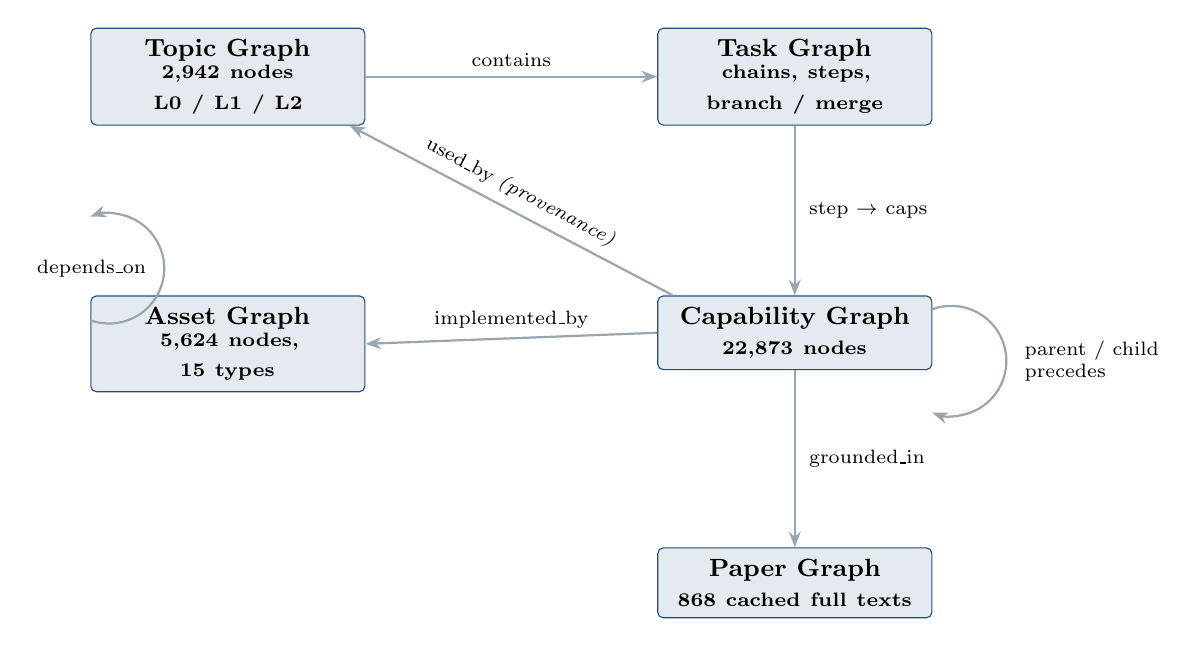
\begin{tikzpicture}[x=1mm,y=1mm]

\node[hdr,text width=32mm,anchor=north west] (topic) at (0,0)
   {Topic Graph\\{\scriptsize 2{,}942 nodes\\L0 / L1 / L2}};
\node[hdr,text width=32mm,anchor=north west] (task) at (72,0)
   {Task Graph\\{\scriptsize chains, steps,\\branch / merge}};
\node[hdr,text width=32mm,anchor=north west] (asset) at (0,-34)
   {Asset Graph\\{\scriptsize 5{,}624 nodes,\\15 types}};
\node[hdr,text width=32mm,anchor=north west] (cap) at (72,-34)
   {Capability Graph\\{\scriptsize 22{,}873 nodes}};
\node[hdr,text width=32mm,anchor=north west] (paper) at (72,-66)
   {Paper Graph\\{\scriptsize 868 cached full texts}};

% top edge
\draw[ar] (topic.east) -- (task.west)
   node[midway,above,font=\scriptsize]{contains};
% task -> capability
\draw[ar] (task.south) -- (cap.north)
   node[midway,right=0.5mm,font=\scriptsize]{step $\rightarrow$ caps};
% capability -> asset
\draw[ar] (cap.west) -- (asset.east)
   node[midway,above,font=\scriptsize]{implemented\_by};
% capability -> paper
\draw[ar] (cap.south) -- (paper.north)
   node[midway,right=0.5mm,font=\scriptsize]{grounded\_in};
% capability -> topic (provenance) : diagonal
\draw[ar] ($(cap.north west)+(2,0)$) -- ($(topic.south east)+(-2,0)$)
   node[midway,above,sloped,font=\scriptsize]{used\_by \emph{(provenance)}};

% self loops
\draw[ar] (cap.east) ++(0,3) arc (110:-110:7mm)
   node[midway,right=1mm,font=\scriptsize,align=left]{parent / child\\precedes};
\draw[ar] (asset.west) ++(0,3) arc (70:290:-7mm)
   node[midway,left=1mm,font=\scriptsize]{depends\_on};
\end{tikzpicture}
\caption{The multi-graph schema. Separating capability hierarchy, capability
ordering and capability implementation into distinct edge families is what makes
graph expansion useful at retrieval time: an expansion can follow exactly the
relation the query intent implies.}
\label{fig:schema}
\end{figure}

\subsection{Entities}

\paragraph{Capability.} A capability is an \emph{ability}, not a tool: a named,
typed unit of engineering competence. Each record carries an opaque identifier,
an English Title-Case canonical name, a mandatory Chinese name, an alias list,
and a description written to a fixed template covering method, object,
prerequisites, inputs, outputs, constraints, performance envelope, applicability,
and explicitly the \emph{boundary against sibling capabilities}. That last
requirement is not cosmetic: sibling-boundary text is what makes deduplication
tractable, because near-duplicate capabilities differ precisely in their
boundaries.

Capabilities are levelled: 43 at L1 (paradigm families), 5{,}576 at L2
(engineering paradigms) and 17{,}213 at L3 (concrete techniques); 41 records
predate the levelling scheme and are unlevelled.

\paragraph{Asset.} An asset is a \emph{thing you can actually obtain}: a
repository, framework, package, pretrained model, dataset, simulator, benchmark,
robot platform, or paper. One GitHub repository is exactly one asset; the
canonical name uses upstream spelling. Table~\ref{tab:assettypes} gives the
distribution.

\begin{table}[htbp]
\centering\small
\caption{Asset type distribution ($n=5{,}624$).}
\label{tab:assettypes}
\begin{tabular}{@{}lr lr lr@{}}
\toprule
Type & $n$ & Type & $n$ & Type & $n$ \\
\midrule
tool         & 1{,}633 & dataset     & 567 & benchmark & 96 \\
framework    & 1{,}251 & ros\_package & 198 & library   & 7 \\
model        & 753 & paper       & 166 & software  & 5 \\
package      & 687 & robot       & 125 & code      & 4 \\
             &     & simulator   & 114 & hardware / other & 6 \\
\bottomrule
\end{tabular}
\end{table}

\paragraph{Task chain.} A task chain is an ordered, possibly branching graph of
steps that accomplishes something. Each step declares the capabilities it
requires. Branch steps carry an explicit \texttt{condition}; merge steps are
flagged. Chains are the bridge between ``what exists'' and ``what to do''.

\subsection{Edge families}

\begin{center}
\small
\begin{tabular}{@{}llr@{}}
\toprule
Edge family & Semantics & Count \\
\midrule
\texttt{parent}/\texttt{child} & capability specialization & 24{,}529 \\
\texttt{precedes}/\texttt{preceded\_by} & ordering within chains & 43{,}973 \\
\texttt{cap}$\rightarrow$\texttt{asset} & implemented by & 31{,}803 \\
\texttt{cap}$\rightarrow$\texttt{topic} (\texttt{used\_by}) & provenance / reuse & 36{,}713 \\
\texttt{context} records & co-step and successor context & 104{,}325 \\
\bottomrule
\end{tabular}
\end{center}

\noindent 17{,}729 capabilities have a parent and 5{,}622 have children, giving a
genuinely deep hierarchy rather than a flat tag cloud. 22{,}501 capabilities
participate in at least one ordering edge.

\subsection{Semantic views}
\label{sec:views}

A single vector per entity is a poor representation, because the name, the
concept, the functional signature, the position in the hierarchy and the
implementation are different kinds of information that dilute each other when
averaged. \eb\ instead decomposes each entity into independently embedded
\textbf{semantic views}: six for capabilities (\emph{identity}, \emph{concept},
\emph{function}, \emph{relation}, \emph{context}, \emph{implementation}), five
for assets, three for topics.

Crucially, three of the six capability views --- relation, context and
implementation --- are synthesized \emph{directly from the graph} at zero LLM
cost: the relation view is the entity's hierarchy neighbourhood, the context view
its dependency neighbourhood, the implementation view its asset set. The function
view is extracted from the description by pattern matching the structured
``input / dependency / output / constraint'' fields that the description template
mandates. This is a concrete payoff of compiling to structure: the graph
\emph{is} additional retrieval signal, obtainable for free.

The live index contains 174{,}189 view vectors (2560-d, fp16, Qwen3-Embedding-4B):
137{,}240 for capabilities, 28{,}120 for assets, 8{,}829 for topics.

% ============================================================
\section{Runtime}
\label{sec:runtime}

The runtime is a consumer of the compiled artifact. Its job is not to understand
robotics; it is to find the right region of the graph and assemble it.

\subsection{Retrieval}

Figure~\ref{fig:retrieval} shows the retrieval stack. Its ordering constraint is
that \textbf{LLM intent decomposition happens before all recall}, so that both the
lexical and dense routes retrieve against the decomposed sub-queries rather than
the raw string.

\begin{figure}[t]
\centering
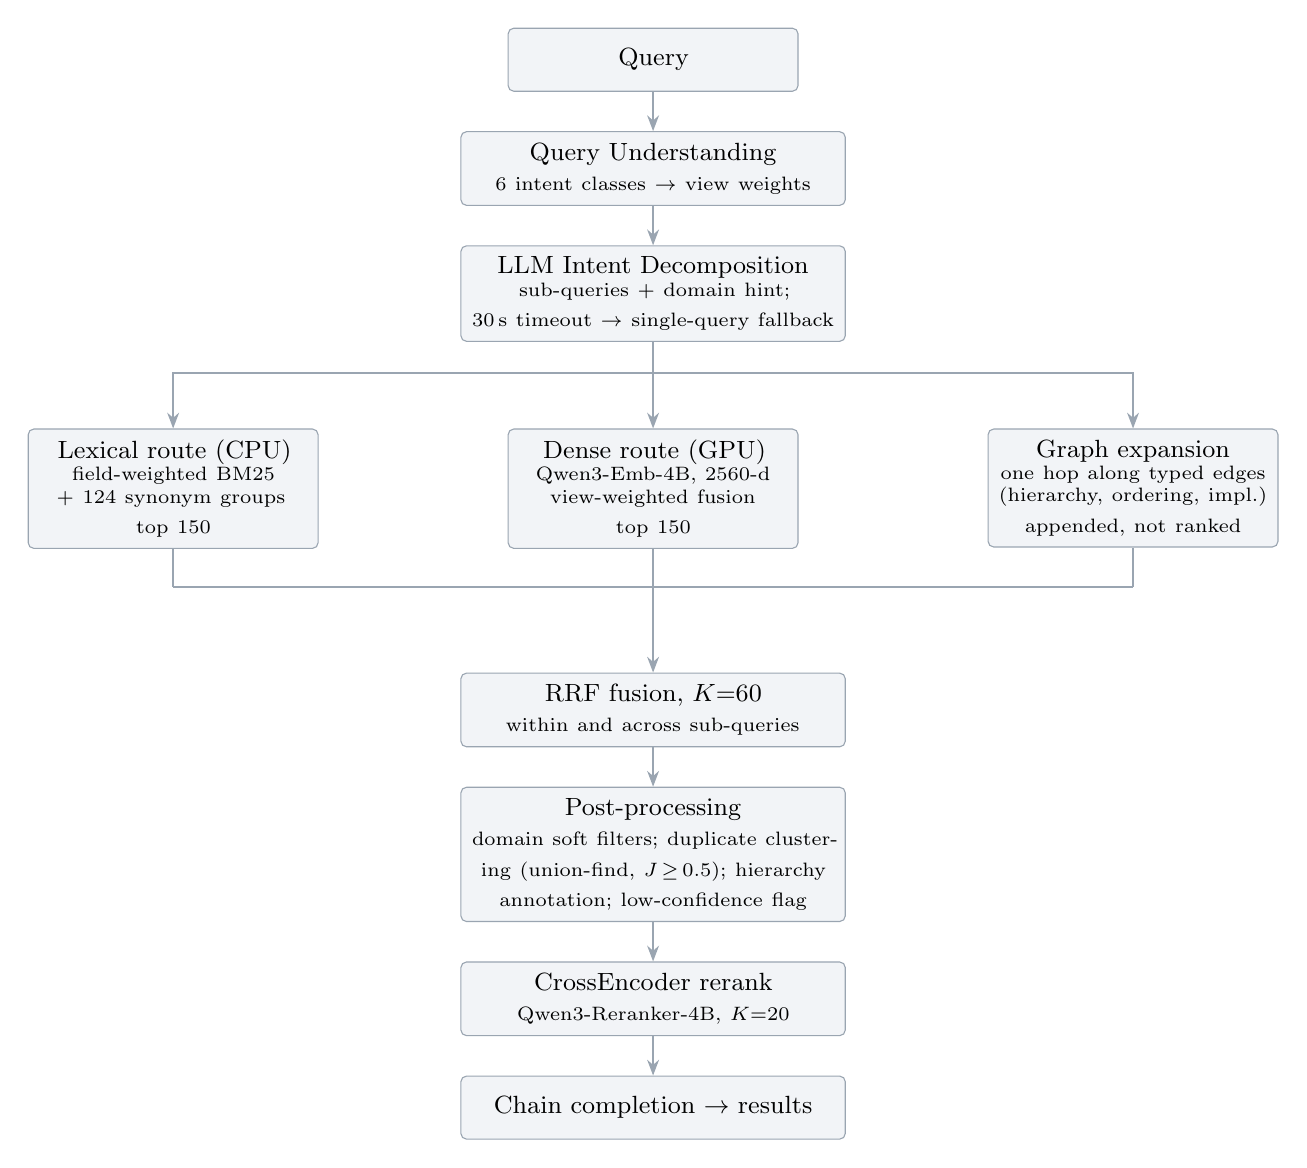
\begin{tikzpicture}[node distance=5mm]
\node[block,text width=34mm] (q) {Query};
\node[block,text width=46mm,below=of q] (qc) {Query Understanding\\{\scriptsize 6 intent classes $\rightarrow$ view weights}};
\node[block,text width=46mm,below=of qc] (plan) {LLM Intent Decomposition\\{\scriptsize sub-queries $+$ domain hint;\\ 30\,s timeout $\rightarrow$ single-query fallback}};

\node[block,text width=34mm,below left=11mm and 18mm of plan] (lex) {Lexical route (CPU)\\{\scriptsize field-weighted BM25\\ $+$ 124 synonym groups\\ top 150}};
\node[block,text width=34mm,below=11mm of plan] (vec) {Dense route (GPU)\\{\scriptsize Qwen3-Emb-4B, 2560-d\\ view-weighted fusion\\ top 150}};
\node[block,text width=34mm,below right=11mm and 18mm of plan] (gex) {Graph expansion\\{\scriptsize one hop along typed edges\\ (hierarchy, ordering, impl.)\\ appended, not ranked}};

\node[block,text width=46mm,below=42mm of plan] (rrf) {RRF fusion, $K{=}60$\\{\scriptsize within and across sub-queries}};
\node[block,text width=46mm,below=of rrf] (post) {Post-processing\\{\scriptsize domain soft filters; duplicate clustering (union-find, $J\!\geq\!0.5$); hierarchy annotation; low-confidence flag}};
\node[block,text width=46mm,below=of post] (rr) {CrossEncoder rerank\\{\scriptsize Qwen3-Reranker-4B, $K{=}20$}};
\node[block,text width=46mm,below=of rr] (out) {Chain completion $\rightarrow$ results};

\draw[ar] (q)--(qc); \draw[ar] (qc)--(plan);
\draw[ar] (plan.south) -- ++(0,-4mm) -| (lex.north);
\draw[ar] (plan.south) -- ++(0,-4mm) -| (vec.north);
\draw[ar] (plan.south) -- ++(0,-4mm) -| (gex.north);
\coordinate (busy) at ($(gex.south)+(0,-5mm)$);
\coordinate (bus) at (rrf.north |- busy);
\draw[draw=ebline,thick] (lex.south) -- (lex.south |- bus);
\draw[draw=ebline,thick] (vec.south) -- (vec.south |- bus);
\draw[draw=ebline,thick] (gex.south) -- (gex.south |- bus);
\draw[draw=ebline,thick] (lex.south |- bus) -- (gex.south |- bus);
\draw[ar] (bus) -- (rrf.north);
\draw[ar] (rrf)--(post); \draw[ar] (post)--(rr); \draw[ar] (rr)--(out);
\end{tikzpicture}
\caption{Three-layer hybrid retrieval. Each signal is scored exactly once; fusion
happens only at the RRF layer, and the final ordering is determined solely by the
cross-encoder.}
\label{fig:retrieval}
\end{figure}

\paragraph{Intent-conditioned view weighting.} The query classifier assigns one of
six intents and selects a corresponding weight profile over the six capability
views (Table~\ref{tab:weights}). Precedence is Relation $>$ Context $>$
Implementation $>$ Function $>$ Identity $>$ Concept; entity-name queries are
detected either by matching the alias/term index or by short-ASCII-name shape.

\begin{table}[htbp]
\centering\small
\caption{Intent-conditioned semantic-view weight profiles (capability scope, normalized).}
\label{tab:weights}
\begin{tabular}{@{}lcccccc@{}}
\toprule
Intent & identity & concept & function & relation & context & implementation \\
\midrule
Identity       & \textbf{0.55} & 0.15 & 0.05 & 0.05 & 0.05 & 0.15 \\
Function       & 0.10 & 0.15 & \textbf{0.50} & 0.05 & 0.10 & 0.10 \\
Relation       & 0.10 & 0.10 & 0.05 & \textbf{0.55} & 0.15 & 0.05 \\
Context        & 0.05 & 0.10 & 0.10 & 0.15 & \textbf{0.55} & 0.05 \\
Implementation & 0.15 & 0.10 & 0.10 & 0.05 & 0.05 & \textbf{0.55} \\
\bottomrule
\end{tabular}
\end{table}

\paragraph{Lexical route.} Per-field BM25 ($k_1{=}1.5$, $b{=}0.75$) with
independent indices so that document-frequency statistics of one field do not
contaminate another. Name carries weight 5.0; exact hits add $+2.0$; contiguous
phrase hits add $1.5\times$ field weight; exact repository matches add 4.0;
character-trigram matching provides spelling tolerance. A 124-group robotics
synonym dictionary (e.g. IK $\leftrightarrow$ Inverse Kinematics) is applied
symmetrically to queries and documents with a token weight of 1.5, which is the
main lever for short Chinese queries where lexical overlap with English canonical
names is zero.

\paragraph{Dense route.} Qwen3-Embedding-4B, 2560 native dimensions, fp16 on GPU,
asymmetric retrieval convention (instruction prefix on the query side only).
The index is a hand-built exact PyTorch index: all vectors live in one
L2-normalized GPU tensor, so cosine similarity is a single matrix multiply.
This was a deliberate trade --- neither FAISS-GPU nor Milvus-GPU is available on
the team's Windows deployment target --- but it also buys exact 100\% recall
(not approximate) and $O(1)$ insert/delete via swap-remove, which matters because
the artifact is continuously recompiled.

\paragraph{Fusion.} Lexical and dense scores are not commensurable, so fusion is
by reciprocal rank~\cite{cormack2009rrf} rather than weighted sum, with two
parameter regimes: $K{=}60$ at the coarse stage (large pool, $\sim$150 per route)
and $K{=}20$ at the fine stage (small pool), where sharper rank discrimination is
wanted. Ties are broken deterministically by dense score, then lexical score,
then identifier, so results are reproducible.

\paragraph{Graph expansion.} For capability hits, a one-hop expansion follows
hierarchy, ordering and implementation edges. Expanded results are appended after
the ranked results and do not consume top-$k$ slots --- they are structural
context, not competing answers.

\subsection{Assembly and gap detection}

The runtime's distinguishing endpoint is not search but \emph{assembly}. Given a
goal, the system retrieves a candidate pool across topics and asks an LLM to
compose one or more executable chains from it, allowing branch and merge. Every
capability identifier the model emits is validated against the pool: an
identifier that does not exist is first fuzzy-matched, and if it still cannot be
resolved it is converted into an explicit \textbf{gap proposal} rather than
silently dropped.

This is the property that a RAG system structurally cannot provide. The answer to
``how do I build this'' is not a paragraph; it is a chain in which every node is
labelled either \emph{owned} (a real capability with real assets) or \emph{gap}
(a required capability nothing in the artifact implements). Gaps are then fed back
as compilation targets, closing the loop in Figure~\ref{fig:arch}.

% ============================================================
\section{Case Study: Compiling \texttt{a\_star\_path\_planning}}
\label{sec:case}

We trace one real compilation unit end to end. The topic
\texttt{a\_star\_path\_planning} sits at L2 under Navigation. It is a useful case
precisely because it looks trivial --- ``$A^\ast$ is a textbook algorithm'' ---
and is not.

\subsection{Input: evidence}

The evidence planner produced a seed query matrix of ten seeds, among them:

\begin{quote}\ttfamily\small
A* path planning robot navigation occupancy grid\\
Hybrid A* Reeds-Shepp car-like vehicle path planning\\
Jump Point Search JPS pathfinding grid Harabor\\
Theta* any-angle path planning Daniel Nash line-of-sight
\end{quote}

\noindent together with a synonym expansion table and an explicit boundary note
excluding the sibling topic
\texttt{cost\_map\_planning}. The resulting chain document enumerates the
paradigm landscape, a representative-systems table with repository URLs and
per-chain attribution, and a key-paper list.

\subsection{Output: four non-equivalent chains}

The compiler did \emph{not} produce ``one $A^\ast$ capability''. It produced four
chains distinguished by state-space representation and expansion rule:

\begin{center}
\small
\begin{tabular}{@{}llll@{}}
\toprule
Chain & State space & Expansion rule & Anchor \\
\midrule
Grid $A^\ast$   & 2-D occupancy cell & 4/8-connected & Hart et al. 1968~\cite{hart1968astar} \\
Hybrid $A^\ast$ & continuous SE(2)   & kinematic primitives, Reeds--Shepp & Dolgov et al. 2008~\cite{dolgov2008hybrid} \\
JPS             & 2-D occupancy cell & look-ahead + jumping rules & Harabor \& Grastien 2011~\cite{harabor2011jps} \\
Theta$^\ast$    & 2-D occupancy cell & line-of-sight parent rewiring & Daniel et al. 2010~\cite{daniel2010theta} \\
\bottomrule
\end{tabular}
\end{center}

\noindent This distinction is exactly the thing a retrieval system does not give
you and an engineer needs first. A car-like robot with non-holonomic constraints
cannot use grid $A^\ast$ at all; a query that returns ``$A^\ast$ is a heuristic
graph search with $f(n)=g(n)+h(n)$'' is not merely incomplete, it is
operationally misleading.

\subsection{Output: capabilities}

Compilation admitted 20 capabilities for this topic: 4 at L2, one per paradigm,
and 16 at L3. Table~\ref{tab:astar} lists them with the assets the implementation
graph attaches to each. Note that the four L2 capabilities are siblings, not
synonyms --- each carries the boundary text that distinguishes it from the other
three, which is what allowed them to survive deduplication as distinct entities.

\begin{table}[htbp]
\centering\small
\caption{Compiled capabilities for the \texttt{a\_star\_path\_planning} topic and
the assets the implementation graph attaches to each, as stored in the live
artifact. Each capability is a distinct registry entity; the surrogate keys are
omitted here for readability.}
\label{tab:astar}
\begin{tabular}{@{}cp{58mm}p{68mm}@{}}
\toprule
Level & Capability & Implementing assets \\
\midrule
\multicolumn{3}{@{}l}{\textit{Chain 1 --- Grid $A^\ast$ (discrete occupancy grid, 4/8-connected)}}\\
L2 & Grid Based $A^\ast$ Path Planning & nav2\_smac\_planner, nav2\_theta\_star\_planner, Hart--Nilsson--Raphael 1968 \\
L3 & Discrete Grid $A^\ast$ Search & PythonRobotics, nav2\_smac\_planner, Hart--Nilsson--Raphael 1968 \\
L3 & Admissible Heuristic Selection for Grid $A^\ast$ & PythonRobotics, nav2\_smac\_planner \\
L3 & Open/Closed Set Management on Grid & PythonRobotics, nav2\_smac\_planner \\
L3 & Obstacle Map Inflation and Collision Check & MoveIt 2, Nav2, nav2\_costmap\_2d, nav2\_smac\_planner, PythonRobotics, SBPL \\
L3 & Path Reconstruction via Parent-Index Backtracking & PythonRobotics, nav2\_smac\_planner \\
\midrule
\multicolumn{3}{@{}l}{\textit{Chain 2 --- Hybrid $A^\ast$ (continuous SE(2), kinematic primitives)}}\\
L2 & Continuous-State Hybrid $A^\ast$ Path Planning & Nav2, navfn, move\_base, Dolgov et al. 2008 \\
L3 & Hybrid $A^\ast$ SE(2) State Node Expansion & PythonRobotics, nav2\_smac\_planner, kfreund/hybrid-a-star, Dolgov et al. 2008 \\
L3 & Reeds--Shepp Curve Shortcut Expansion & PythonRobotics, nav2\_smac\_planner, kfreund/hybrid-a-star \\
L3 & Motion Primitive Steer Set Discretization & PythonRobotics, nav2\_smac\_planner, kfreund/hybrid-a-star \\
L3 & Vehicle Footprint Continuous Collision Check & PyBullet, Box2D, Jolt Physics, PythonRobotics, nav2\_smac\_planner \\
L3 & Hybrid $A^\ast$ 2D Reverse Heuristic & nav2\_smac\_planner \\
\midrule
\multicolumn{3}{@{}l}{\textit{Chain 3 --- Jump Point Search (symmetry pruning on the same grid)}}\\
L2 & Jump Point Search Grid $A^\ast$ Optimization & Harabor--Grastien 2011 \\
L3 & JPS Look-ahead Rule Pruning & hjandroid/JumpPointSearch, qiao/PathFinding.js \\
L3 & JPS Jumping Rule Recursive Expansion & hjandroid/JumpPointSearch, qiao/PathFinding.js, Harabor--Grastien 2011 \\
L3 & Forced Neighbor Detection & hjandroid/JumpPointSearch, qiao/PathFinding.js \\
\midrule
\multicolumn{3}{@{}l}{\textit{Chain 4 --- Theta$^\ast$ (any-angle, line-of-sight rewiring)}}\\
L2 & Any-Angle Theta$^\ast$ Path Planning & nav2\_theta\_star\_planner, PythonRobotics, Daniel et al. 2010 \\
L3 & Theta$^\ast$ Line-of-Sight Bresenham Check & nav2\_theta\_star\_planner, PythonRobotics, Daniel et al. 2010 \\
L3 & Theta$^\ast$ Parent Rewiring Path Compression & nav2\_theta\_star\_planner, PythonRobotics, Daniel et al. 2010 \\
\bottomrule
\end{tabular}
\end{table}

\subsection{What the compiled record actually contains}

The stored description for \emph{Grid Based $A^\ast$ Path Planning} is not a
summary. Rendered from
its template it declares: the procedure (obstacle inflation $\rightarrow$
open/closed set initialization $\rightarrow$ heuristic evaluation $\rightarrow$
4/8-connected main loop $\rightarrow$ parent-index backtracking); the optimality
condition ($f(n)=g(n)+h(n)$ is optimal when $h$ is admissible); the applicability
split (4-connected for Manhattan motion, 8-connected for omnidirectional);
prerequisites (discrete grid map, start and goal); inputs (obstacle point set,
endpoints, robot radius); outputs (grid waypoint sequence); constraints
(admissible heuristic, single-source single-sink); a performance envelope
(millisecond scale on a $100\times100$ grid); and canonical implementations.

This is the difference the compiler makes. Each field is separately embedded as a
semantic view, separately retrievable, and separately consumable by a downstream
planner.

\subsection{Reuse}

\emph{Obstacle Map Inflation and Collision Check} is a good
illustration of the linker at work. It was minted once during this compilation
and is now referenced by eight distinct L2 topics:

\begin{quote}\ttfamily\small
a\_star\_path\_planning \quad adaptive\_coverage\_path\\
chance\_constrained\_navigation \quad configuration\_space\_planning\\
safety\_margin\_planning \quad topological\_graph\_representation\\
uncertainty\_aware\_planning \quad underwater\_obstacle\_avoidance
\end{quote}

\noindent It links to six assets spanning
navigation, manipulation and search-based planning stacks. A per-topic document
generator would have written eight unrelated paragraphs; the compiler wrote one
node with eight inbound provenance edges. Across the whole artifact, 6{,}533 capabilities (28.6\%) are used by
more than one topic, over 36{,}713 capability--topic usages.

% ============================================================
\section{Measurements and Evaluation Infrastructure}
\label{sec:eval}

Table~\ref{tab:stats} reports the state of the live compiled artifact. We
emphasize that these are inventory and structural statistics, not a benchmark
result; \S\ref{sec:limits} discusses what we do not yet measure.

\begin{table}[htbp]
\centering\small
\caption{Compiled artifact statistics. Entity counts are a live registry snapshot (2026-07-29); edge counts are from the derived graph indices (2026-07-27) restricted to entities present in the live registry, so every edge endpoint resolves.}
\label{tab:stats}
\begin{tabular}{@{}llr@{}}
\toprule
Category & Quantity & Value \\
\midrule
\multirow{3}{*}{Taxonomy}
 & L0 domains & 15 \\
 & L1 sub-domains & 416 \\
 & L2 compilation units & 2{,}511 \\
\midrule
\multirow{5}{*}{Progress}
 & L2 topics with a compiled record on disk & 1{,}740 (69.3\%) \\
 & L2 topics represented in the graph indices & 1{,}605 (63.9\%) \\
 & L2 topics not yet compiled & 771 \\
 & Topic directories with evidence documents & 1{,}698 \\
 & Chain evidence documents & 5{,}510 (3.24 / topic) \\
\midrule
\multirow{4}{*}{Entities}
 & Capabilities & 22{,}873 \\
 & \quad L1 / L2 / L3 & 43 / 5{,}576 / 17{,}213 \\
 & Assets & 5{,}624 (15 types) \\
 & Cached arXiv full texts & 868 \\
\midrule
\multirow{5}{*}{Edges}
 & Hierarchy (parent$\rightarrow$child) & 24{,}529 \\
 & Ordering (precedes) & 43{,}973 \\
 & Implementation (cap$\rightarrow$asset) & 31{,}803 \\
 & Provenance (cap$\rightarrow$topic) & 36{,}713 \\
 & Context records & 104{,}325 \\
\midrule
\multirow{3}{*}{Structure}
 & Capabilities with a parent & 17{,}729 (77.5\%) \\
 & Capabilities with children & 5{,}622 (24.6\%) \\
 & Capabilities reused across topics & 6{,}533 (28.6\%) \\
\midrule
\multirow{3}{*}{Grounding}
 & Capabilities with $\geq 1$ asset & 15{,}689 (68.6\%) \\
 & \quad by level: L1 / L2 / L3 & 32.6\% / 47.7\% / 75.5\% \\
 & Mean assets per grounded capability & 2.03 \\
\midrule
\multirow{4}{*}{Index}
 & Semantic view vectors & 174{,}189 \\
 & \quad capabilities / assets / topics & 137{,}240 / 28{,}120 / 8{,}829 \\
 & Encoder & Qwen3-Embedding-4B, 2560-d, fp16 \\
 & Synonym groups & 124 \\
\midrule
\multirow{2}{*}{Quality control}
 & Suspect pairs: resolved / merged / open & 1{,}116 / 39 / 43 \\
 & Peak unadjudicated backlog (historical) & 2{,}527 \\
\bottomrule
\end{tabular}
\end{table}

\paragraph{Coverage is a progress reading, not a ceiling.} The compiler is
running --- the topic-record count rose by one during the measurement run that
produced this section. At the time of measurement 1{,}740 of 2{,}511 L2 topics
(69.3\%) had a compiled record on disk, leaving 771 uncompiled.

Two coverage figures appear in Table~\ref{tab:stats} because they measure
different things, and we report both rather than picking the flattering one:
1{,}740 records exist on disk, while the derived graph indices attribute
capabilities to 1{,}605 distinct topics. The gap is index lag --- records are
written continuously and the indices are rebuilt periodically --- and it is the
same lag that explains the 11\% discrepancy between the two independent
amortization estimates in \S\ref{sec:outputmeasure}. We note additionally that
the pipeline's own run ledger reported a lower figure (1{,}081) than a direct
disk scan; the ledger is a cache and the file system is authoritative, which is
what the orchestration specification itself asserts.

\paragraph{Reading the numbers.} Three of the remaining figures carry most of the
signal.

First, \textbf{grounding rate rises with specificity}: 75.5\% of L3 capabilities
have at least one concrete implementing asset, versus 47.7\% at L2 and 32.6\% at
L1. This is the expected and desirable shape --- an abstract paradigm is not
supposed to have a repository, a concrete technique is --- and it is a
sanity check on level assignment.

Second, \textbf{reuse is the metric that distinguishes a compiler from a document
generator}. An earlier internal audit (2026-07) found that roughly 96\% of
capabilities were referenced by exactly one topic, i.e. the system was mostly
producing per-topic documents that happened to share a schema. Under the current
registry-candidate-injection and deduplication regime that figure has moved to
71.6\% single-topic / 28.6\% multi-topic. Reuse is the direct measure of whether
the symbol table is doing its job, and it is the metric we optimize.

Third, \textbf{the suspect ledger is a control-system reading, not a defect
count}. A backlog of 2{,}527 was not evidence of a dirty knowledge base; it was
evidence of an unbounded queue with no consumer. Settling suspects inside each
compilation transaction bounded the queue: 43 open pairs against 22{,}873
capabilities.

\subsection{Evaluating the deduplication gate}
\label{sec:gateeval}

The adjudicated duplicate ledger is a labelled dataset: every entry records the
similarity score that flagged the pair, the metric that produced it, and the
adjudicated outcome. Treating \textsf{merged} as ``true duplicate'' and
\textsf{resolved} as ``not a duplicate'' gives 1{,}155 labelled pairs, which lets
us ask a question the system's design implicitly answers but never tested: once a
pair has been flagged, \emph{does the similarity score carry information about
whether it is actually a duplicate?}

\paragraph{Scope, stated first.} These pairs are exactly those that already
passed the gate, so the measurement is conditional on being flagged. It does not
estimate the gate's overall discriminative power over all pairs, and we do not
report it as such. It answers the narrower and operationally decisive question:
should the score influence the decision \emph{after} flagging?

\paragraph{Result.} It should not. Table~\ref{tab:gate} reports precision at the
operating threshold and the area under the ROC curve using similarity as the
duplicate score, with bootstrap confidence intervals over 2{,}000 resamples.

\begin{table}[htbp]
\centering\small
\caption{Deduplication gate evaluated on 1{,}155 adjudicated pairs. AUC uses the
similarity score as a duplicate detector \emph{within the flagged set}; 0.5 is
chance.}
\label{tab:gate}
\begin{tabular}{@{}lrrrcc@{}}
\toprule
Path & pairs & true dup. & precision & AUC & 95\% CI \\
\midrule
Embedding (primary) & 508 & 35 & 0.069 & 0.629 & [0.531, 0.722] \\
Lexical (fallback)  & 647 &  4 & 0.006 & 0.454 & [0.271, 0.764] \\
\bottomrule
\end{tabular}
\end{table}

The embedding path carries weak but statistically detectable signal --- its
confidence interval excludes chance --- and is nonetheless far too weak to serve
as a decision rule: 93\% of what it flags is not a duplicate. The lexical
fallback path has a point estimate \emph{below} chance, but with only four
positive examples its interval spans almost the entire range; we report it for
completeness and draw no conclusion from it beyond the obvious one, that a
fallback path exercised this rarely cannot be validated from production data.

\paragraph{Tuning does not fix this.} The natural response is to raise the
threshold. Figure~\ref{fig:gate} shows what that buys. Moving the operating point
from $0.86$ to $0.94$ raises precision from 0.069 to 0.126 --- still one true
duplicate in eight --- while discarding half the true duplicates. Beyond $0.95$
the curve becomes noise-dominated on single-digit counts. There is no operating
point at which the score alone is a usable decision procedure.

\begin{figure}[htbp]
\centering
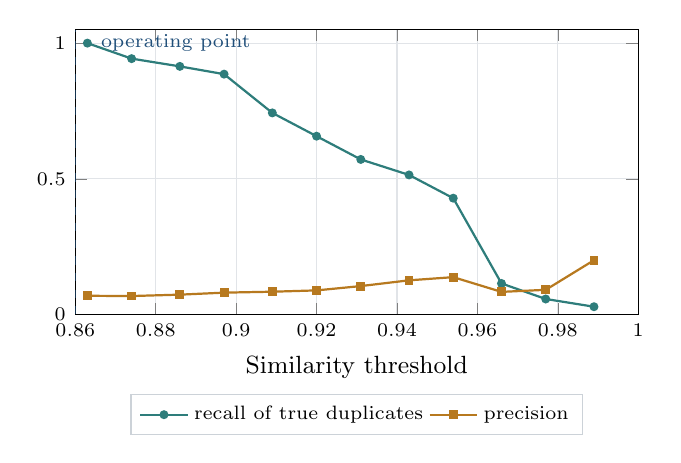
\begin{tikzpicture}
\begin{axis}[
  width=0.72\textwidth, height=5.2cm,
  xlabel={Similarity threshold}, ylabel={},
  xmin=0.86, xmax=1.0, ymin=0, ymax=1.05,
  grid=major, grid style={draw=ebline!30},
  tick label style={font=\scriptsize}, label style={font=\small},
  legend style={font=\scriptsize, at={(0.5,-0.28)}, anchor=north, legend columns=2, draw=ebline!50},
]
\addplot[color=ebteal, thick, mark=*, mark size=1.2pt] coordinates {
(0.863,1.0000) (0.874,0.9429) (0.886,0.9143) (0.897,0.8857) (0.909,0.7429)
(0.920,0.6571) (0.931,0.5714) (0.943,0.5143) (0.954,0.4286) (0.966,0.1143)
(0.977,0.0571) (0.989,0.0286)};
\addlegendentry{recall of true duplicates}
\addplot[color=ebamber, thick, mark=square*, mark size=1.2pt] coordinates {
(0.863,0.0689) (0.874,0.0680) (0.886,0.0731) (0.897,0.0805) (0.909,0.0839)
(0.920,0.0888) (0.931,0.1047) (0.943,0.1259) (0.954,0.1376) (0.966,0.0833)
(0.977,0.0909) (0.989,0.2000)};
\addlegendentry{precision}
\addplot[color=ebblue, dashed, thick, forget plot] coordinates {(0.86,0) (0.86,1.05)};
\node[font=\scriptsize, text=ebblue, anchor=west] at (axis cs:0.864,1.0) {operating point};
\end{axis}
\end{tikzpicture}
\caption{Threshold sweep for the embedding deduplication path within the flagged
set. Raising the threshold trades away true duplicates far faster than it buys
precision; past $0.95$ the counts fall to single digits and the estimates become
unstable. The design consequence is that the gate cannot be made into a decision
rule by tuning.}
\label{fig:gate}
\end{figure}

\paragraph{What this justifies.} The system's two-stage design --- a
recall-oriented threshold followed by a conservative adjudication stage that is
instructed to answer ``different'' under uncertainty --- was originally adopted on
the argument that false merges are irreversible. This measurement converts that
argument from a design preference into a requirement. The adjudication stage is
not a safety margin on top of a working classifier; it is doing essentially all
of the discrimination. Any system that flags near-duplicate entities by embedding
similarity and then \emph{merges automatically above a threshold} would, at our
operating point, be wrong more than nine times in ten.

We regard this as the most transferable empirical result in the paper, and note
that it is only measurable because adjudication decisions were recorded with
their scores and rationales rather than applied and forgotten.

\subsection{Compilation output: structure, provenance and refusal}
\label{sec:outputmeasure}

Three further measurements over the full set of 1{,}740 compiled topic records
(the compiler was running during measurement; counts drift upward by a few
records per hour).

\paragraph{Chain structure.} The 1{,}740 records contain 5{,}756 task chains
(3.31 per topic) with 11.07 steps per chain on average (median 10, p90 16). Of
these, 22.8\% contain a branch, 22.2\% contain an explicit merge node, and
\textbf{74.1\% are purely linear}. An earlier internal audit had estimated 69\%;
the full-corpus figure is slightly worse. Since the schema supports branching and
the validator does not require it, this is an extraction-incentive problem: the
compiler produces the simplest structure that passes, and nothing rewards
capturing genuine route divergence. It is the clearest quality deficit we can
currently measure.

\paragraph{Provenance integrity.} Every topic record cites the chain research
documents it was assembled from. Because those documents are files, the citation
can be checked mechanically. Of 5{,}545 chain-document references, \textbf{98.29\%
resolve to a file that exists}; 95 are broken, and 58 records (3.3\%) carry no
chain-document reference at all. Of the topic-level research document references,
5 are broken.

We propose this as a metric for LLM-constructed knowledge graphs generally.
Structural validity is routinely checked; \emph{provenance resolvability} --- the
fraction of an artifact's own evidence citations that actually resolve --- is not,
and it is cheap to compute, hard to game, and directly diagnostic of whether a
pipeline's evidence layer is real or decorative. A system that cannot report it
has no evidence layer to speak of.

\paragraph{Refusal to fabricate.} The specification requires that an unverifiable
field be marked unverified rather than filled in, and treats inventing a citation
as a more serious failure than leaving a gap. That instruction is followed:
1{,}105 unverified markers survive in the compiled artifact, distributed over
16.2\% of topic records (mean 0.64 per record). We report this deliberately as a
\emph{positive} indicator. The alternative --- zero unverified markers --- would
not indicate a better artifact; given what is actually verifiable about
fast-moving open-source projects, it would indicate a pipeline that fills gaps
rather than declaring them.

\paragraph{Deduplication, seen from the records.} The 1{,}740 records contain
40{,}834 capability entries and 18{,}110 asset entries, which the registry
collapses to 22{,}873 and 5{,}624 distinct entities respectively --- a
$1.79\times$ collapse for capabilities and $3.22\times$ for assets. The
capability figure is an independent estimate of the amortization factor of
\S\ref{sec:amort}, arrived at by counting record entries rather than provenance
edges, and it agrees with the edge-derived estimate ($1.61$) to within 11\%. The
residual gap is provenance-edge lag: the graph indices are rebuilt periodically
while records are written continuously.

\subsection{Retrieval evaluation: the harness, and the state of its results}
\label{sec:golden}

Retrieval quality cannot be inferred from inventory statistics, so we built a
domain-specific evaluation suite. We describe its design here as a methodological
contribution, and then state plainly that we do not currently have a valid result
from it.

\paragraph{The golden set.} 126 queries across eight intent classes
(Table~\ref{tab:golden}), written in the mixed Chinese/English register that
actual users of a robotics knowledge base type. Three properties distinguish it
from a naive relevance set.

First, \textbf{assertions come in three strengths}, because not every query has a
single correct entity. \texttt{expect} names exact identifiers; \texttt{expect\_any}
accepts any member of a set, which is the honest form for a query like ``detect
the cup on the table and generate a grasp pose'' that legitimately spans two
entities; and \texttt{expect\_match} is a structural predicate --- for example,
\emph{a result anchored to topic \texttt{a\_star\_path\_planning} whose text
contains ``heuristic''} --- which is the only workable form for mechanism
questions whose answer lives in a chain document or a step card rather than in an
entity description.

Second, it carries \textbf{negative assertions}. \texttt{reject} and
\texttt{reject\_match} declare what must \emph{not} be retrieved, and the
false-recall rate is reported alongside recall. The most instructive of these
takes a literal web-search query string lifted from a chain document's retrieval
ledger --- text that looks exactly like a technical question --- and asserts that
it must not retrieve any retrieval-log section. That is a test that the evidence
index does not leak its own provenance metadata back as content, and it is the
kind of failure that only a system with a provenance layer can have.

Third, the set is \textbf{regenerated rather than maintained}. Identifiers are
surrogate keys that change under registry rebuilds, so the checked-in golden file
is a build product: the maintained source names entities by name, and a build step
resolves names to current identifiers. This is the same names-versus-keys
discipline as \S\ref{sec:order}, applied to test data. Several entries carry
annotations recording the audit that motivated them --- for instance a query
whose Chinese phrasing was found to be misclassified into the wrong intent class
--- so the suite accumulates regressions rather than only covering the happy path.

\begin{table}[htbp]
\centering\small
\caption{Golden set composition ($n=126$). Assertion counts overlap with intent
classes; six queries are diagnostic only and carry no positive assertion.}
\label{tab:golden}
\begin{tabular}{@{}lr@{\hspace{8mm}}lr@{}}
\toprule
Intent class & $n$ & Assertion form & $n$ \\
\midrule
identity     & 34 & \texttt{expect} (exact ids)        & 34 \\
concept      & 25 & \texttt{expect\_any} (any-of set)  & 49 \\
function     & 15 & \texttt{expect\_match} (predicate) & 37 \\
selection    & 15 & \texttt{reject} (must not retrieve) & 8 \\
evidence     & 13 & \texttt{reject\_match}              & 5 \\
io           & 10 & & \\
multihop     &  7 & & \\
negative     &  7 & & \\
\bottomrule
\end{tabular}
\end{table}

\paragraph{The harness.} The evaluation driver reports nDCG@10, recall@20, MRR,
false-recall rate against the negative assertions, and latency at the 50th, 95th
and 99th percentiles --- broken down by intent class, which matters because the
retrieval stack conditions its view weighting on exactly that classification
(\S\ref{sec:runtime}) and a stack that is strong on identity queries and weak on
mechanism queries would otherwise average out to something unremarkable.

\paragraph{What we do not have.} We have no valid current run. The most recent
execution recorded a complete failure --- all 126 queries failed with zero
latency, the signature of the vector service being unavailable rather than of
poor retrieval --- and the last successful run predates the surrogate-key
migration, covers only six queries, and asserts against identifiers that no
longer exist. We therefore report no retrieval numbers in this paper. The
apparatus is built and the gap is an execution gap rather than a research one;
we will publish results, and the suite itself, separately.

\begin{table}[htbp]
\centering\small
\caption{Retrieval evaluation: metrics the harness reports, awaiting a valid run.
We show the empty table deliberately, to be unambiguous about what is and is not
claimed in this paper.}
\label{tab:evalpending}
\begin{tabular}{@{}lcccccc@{}}
\toprule
Intent class & $n$ & nDCG@10 & recall@20 & MRR & false-recall & p95 latency \\
\midrule
identity & 34 & --- & --- & --- & --- & --- \\
concept & 25 & --- & --- & --- & --- & --- \\
function & 15 & --- & --- & --- & --- & --- \\
selection & 15 & --- & --- & --- & --- & --- \\
evidence & 13 & --- & --- & --- & --- & --- \\
io / multihop / negative & 24 & --- & --- & --- & --- & --- \\
\midrule
\textbf{overall} & \textbf{126} & --- & --- & --- & --- & --- \\
\bottomrule
\end{tabular}
\end{table}

% ============================================================
\section{Discussion: What \eb\ Is Not}
\label{sec:discussion}

It is easy to place a system like this in the wrong category, so we state the
distinctions directly.

\paragraph{Not a search engine.} A search engine returns documents ranked by
relevance to a string. \eb\ returns typed entities with declared inputs, outputs,
prerequisites and implementations, plus the edges between them. The output is
intended for a program, not a reader.

\paragraph{Not a RAG system.} RAG derives structure at query time and discards
it. \eb\ derives structure at compile time and keeps it. A RAG system asked the
same question a thousand times performs the analysis a thousand times and can
give a thousand mutually inconsistent answers; a compiler performs it once and
serves the same artifact. Concretely: our compilation of
\texttt{a\_star\_path\_planning} into four non-equivalent paradigms is a durable
fact in the graph, not a lucky generation.

\paragraph{Not a vector database.} A vector database is a component of our
runtime, not the system. The interesting content of \eb\ is the typed edge
families --- hierarchy, ordering, implementation --- which are what let graph
expansion, chain completion and gap detection work. Vectors alone give you
neighbours; they do not give you \emph{precedes}.

\paragraph{Not an execution ontology.} \eb\ does not model action semantics,
object affordances or robot state in the sense of KnowRob~\cite{tenorth2013knowrob}
or IEEE 1872~\cite{ieee1872}. It models engineering decisions. We view these as
complementary layers and consider the interface between them --- compiled
capability $\rightarrow$ executable action description --- an important
direction, and one that RCDS (\S\ref{sec:rcds}) is intended to make mechanical
rather than manual.

\paragraph{Not classical knowledge compilation.} As stated in
\S\ref{sec:intro}, we do not claim the tractability guarantees of the
OBDD/d-DNNF line of work~\cite{darwiche2002kcmap}. Our compilation target is a
typed property graph, and our ``tractability'' claim is empirical and much
weaker: queries that would require multi-step LLM derivation over raw text become
graph traversals plus retrieval.

\subsection{Beyond the graph: a description standard and a trust ladder}
\label{sec:rcds}

A compiled capability graph answers ``what exists and what implements it''. It
does not yet answer ``can I trust this, and will it compose with what I already
have''. Two mechanisms extend the artifact toward those questions.

\paragraph{RCDS.} The Robot Capability Description Schema is a proposed
specification for describing a robot capability in composable terms: declared
inputs and outputs, service-level expectations, certification status, and the
interface fields required for composition. The purpose is mechanical: with a
shared schema, a planner can automatically check whether two capabilities are
data-flow compatible before proposing that they be chained, instead of leaving
that check to a human reading two READMEs. The schema is what turns a graph of
descriptions into a graph of \emph{composable} units. We regard standardization
here as the durable contribution --- a shared description format outlives any
particular graph built with it.

\paragraph{A three-level evidence ladder.} Capability claims are not equally
trustworthy, and collapsing them onto one axis is how knowledge bases lose
credibility. We distinguish three levels: \textbf{L1}, benchmark performance on a
standard dataset, which reflects theoretical capability; \textbf{L2}, results in
a simulation environment such as Isaac or MuJoCo; and \textbf{L3}, validated
deployment on real hardware in a production setting, including sustained
operating data. The point is not that L3 supersedes L1 --- for many purposes a
dataset number is exactly what you want --- but that a consumer of the graph must
be able to see \emph{which kind} of evidence backs a claim. This ladder is
orthogonal to the compilation gates: those govern structural admission, the
ladder governs epistemic weight.

\paragraph{System layering.} The compiler is one layer of three. Layer 1 is the
compiler described in this paper. Layer 2 is the engine: retrieval, reasoning,
task decomposition and planning over the artifact (\S\ref{sec:runtime}). Layer 3
is the application surface --- question answering, agent and MCP access, and
capability composition. This paper is about Layer 1, because Layer 1 is what the
other two are impossible without.

\paragraph{The positioning claim.} We contend that source-level knowledge
compilation is a missing \emph{infrastructure layer} for robot foundation models,
sitting between the open literature and the model in the same way that a package
registry sits between source code and an application. Models will keep improving.
The knowledge they need to be grounded in will keep being published as prose.
Something has to compile it.

% ============================================================
\section{Limitations and Future Work}
\label{sec:limits}

We list what does not work, because a system paper that reports only successes is
not useful to anyone.

\paragraph{Provenance coverage is partial.} The retrieval-ledger regime described
in \S\ref{sec:evidence} --- enforced search/fetch floors, per-query accounting,
negative-results tables, script-verified repositories --- is the current standard,
but roughly 44\% of chain documents in our sample carry a full ledger. The
remainder were compiled under an earlier regime that did not enforce it. Those
records are structurally valid and were not fabricated, but they are not
\emph{auditable} to the same standard, and we do not claim they are. Re-compiling
them under the current regime is queued work, not a research problem.

\paragraph{Structural validity is guaranteed; factual accuracy is not.} The
structural and registry gates guarantee that the graph is well-formed, that identifiers resolve, that there are
no cycles and that entities are globally unique. They do not guarantee that a
capability's stated performance envelope is correct. The evidence ledger makes
factual claims \emph{traceable} --- which is a precondition for verification, not
a substitute for it. We do not yet run systematic post-hoc factual audit against
primary sources, and expert spot-checking at 22{,}873 capabilities is not
tractable manually. Automated cross-verification (does the cited repository
actually expose the claimed module? does the cited paper actually state the
claimed bound?) is the most important open item.

\paragraph{Grounding coverage is incomplete.} 31.4\% of capabilities have no
attached asset and carry only an inline implementation hint. Those hints are not
structured, not comparable, and not reusable. The gap is concentrated at higher
abstraction levels, which is partly correct by design and partly a real hole.

\paragraph{Reuse is still low.} 28.6\% multi-topic reuse is a large improvement
over the 4\% of the earlier audit but is still far from where a well-linked graph
should be. Some of the residual is genuine (many L3 techniques really are
topic-specific); some is unresolved near-duplication that our deliberately
conservative adjudication policy declines to merge.

\paragraph{Chains are under-branched.} Measured over the full corpus,
74.1\% of task chains are purely linear (\S\ref{sec:outputmeasure}), even though
the schema supports branching, merging and sub-chain references. The validator
does not require branching and the extractor does not volunteer it, so the
compiler emits the simplest structure that passes. This is a
prompt-and-incentive problem rather than a schema problem, and it is the quality
deficit we would attack first.

\paragraph{The central comparison has not been run.} We have argued for
compilation and quantified its amortization (\S\ref{sec:why}), but we have not
demonstrated that a compiled artifact produces better answers than a strong
query-time baseline. The experiment we owe the reader is a head-to-head against
naive RAG and GraphRAG over the same source corpus, measuring answer correctness,
hallucination rate, coverage, end-to-end latency and total cost of ownership
including build cost --- the last of which is the honest way to account for a
system that front-loads work. We do not report it because it does not exist yet,
and reporting a comparison we have not run would be worse than reporting none.

What stands between us and that experiment is smaller than it was. The
domain-specific golden set exists (\S\ref{sec:golden}); what is missing is a
valid run of it, and the baselines to run beside it. The remaining hard
requirement is instrumentation: the pipeline records no per-topic compilation
time or token cost, so build-side economics --- the exact quantity that decides
whether front-loading is worth it --- cannot currently be reported at all. That
is a logging change, not a research question, and it is the single cheapest thing
we could do to strengthen the argument of this paper.

\paragraph{The gate evaluation is small and conditional.} \S\ref{sec:gateeval}
rests on 35 positive examples for the embedding path and four for the lexical
fallback, and is conditioned on pairs that were already flagged. The embedding
result is stable enough to act on --- the confidence interval excludes chance and
the threshold sweep is monotone over the range that matters --- but the lexical
result is not a finding, and neither speaks to the gate's recall: we cannot
measure the duplicates the gate never flagged, because nothing labelled them. A
proper recall estimate requires adjudicating a random sample of \emph{unflagged}
pairs, which we have not done.

\paragraph{Encoder is not domain-adapted.} Qwen3-Embedding-4B is a general model.
Robotics terminology (dense acronyms, repository names, mathematical notation) is
plausibly not well separated in its embedding space, which bounds both retrieval
and deduplication precision. Domain-adaptive fine-tuning on the compiled artifact
itself is a natural next step --- and one the artifact uniquely enables, since it
provides typed positive and hard-negative pairs at scale.

\paragraph{Description templating introduces noise.} Enforcing a description
template improves parseability but induces formulaic phrasing, which adds
lexical and semantic noise to retrieval. Balancing template compliance against
descriptive distinctiveness is unresolved.

\paragraph{Synonym expansion is exact-group only.} The 124 synonym groups match
true synonyms. Broad-concept expansion (SLAM $\rightarrow$ loop closure, pose
graph, scan matching) is not yet implemented; the graph contains exactly this
information and should supply it.

\paragraph{Multilingual scope.} Entities carry both English and Chinese canonical
names by schema, so the graph is bilingual by construction and further languages
require only additional name fields, not schema or relation changes. Full
bilingual coverage of long-form descriptions is not yet complete.

% ============================================================
\section{Conclusion}

The constraint on embodied AI is increasingly the availability of \emph{structured}
engineering knowledge rather than model capacity. Retrieval-augmented generation
addresses the symptom --- getting relevant text in front of a model --- while
leaving the underlying problem untouched: the structure is re-derived on every
query, in prose, without identity or persistence.

\eb\ takes the other approach. It compiles heterogeneous robotics sources into a
persistent typed artifact through a gated pipeline, treats the LLM as an
untrusted parser subject to admission control, and exposes the artifact to a
runtime that can assemble executable capability chains and name what is missing.
The artifact as of this snapshot --- 22{,}873 capabilities, 5{,}624 assets, over
100{,}000 typed edges and 174{,}189 semantic-view vectors, drawn from 1{,}605
topics, with 1{,}430 more queued and the compiler still running --- is large
enough to indicate that the approach scales. It is also, deliberately, a snapshot
of something in motion: the claim we are making is about the pipeline, not about
the size of yesterday's output.

\textbf{Compile Once, Execute Everywhere.}

% ============================================================
\section*{Availability}

The paper, the public indices of the compiled artifact, the retrieval golden set,
the adjudicated deduplication ledger and the measurement script are published at
\url{https://chenli-yy.github.io/entropy-box-public/}, together with interactive views of
the topic graph and the capability dependency network and one topic reproduced in
full. All data is released under CC BY 4.0 and the code under MIT.

A read-only retrieval API over the evidence corpus is open and requires no
registration or client software:

\begin{quote}\ttfamily\small
POST <api-base>/api/evidence/search\\
\{ "query": "...", "top\_k": 10, "mode": "hybrid", "rerank": true \}
\end{quote}

\noindent The current API base URL is listed on the project page above. The same
endpoint is packaged as an Agent Skill declaration and as an MCP stdio server, so
that external agents can query the artifact directly. The
open endpoint currently exposes concept-level evidence retrieval; complex
task retrieval, chain assembly and node-level graph queries are implemented but
not yet exposed as an API, and are reachable through the web interface.

We intend to release the taxonomy, the RCDS specification, an English snapshot of
the capability and asset registries, and a retrieval benchmark.

\section*{Acknowledgements}

The compilation pipeline, the artifact and this paper are the work of a very
small team. We thank the maintainers of the open-source robotics projects that
constitute most of the asset graph --- in particular Nav2, MoveIt, PythonRobotics
and the wider ROS ecosystem --- whose documentation quality is what made
automated compilation feasible at all.

\begin{thebibliography}{99}
\small

\bibitem{ahn2022saycan}
M.~Ahn et al.
\newblock Do As I Can, Not As I Say: Grounding Language in Robotic Affordances.
\newblock \emph{arXiv:2204.01691}, 2022.

\bibitem{auer2007dbpedia}
S.~Auer, C.~Bizer, G.~Kobilarov, J.~Lehmann, R.~Cyganiak, and Z.~Ives.
\newblock DBpedia: A Nucleus for a Web of Open Data.
\newblock In \emph{ISWC/ASWC}, 2007.

\bibitem{beetz2010cram}
M.~Beetz, L.~M{\"o}senlechner, and M.~Tenorth.
\newblock CRAM --- A Cognitive Robot Abstract Machine for Everyday Manipulation
  in Human Environments.
\newblock In \emph{IEEE/RSJ IROS}, 2010.

\bibitem{brohan2023rt2}
A.~Brohan et al.
\newblock RT-2: Vision-Language-Action Models Transfer Web Knowledge to Robotic
  Control.
\newblock \emph{arXiv:2307.15818}, 2023.

\bibitem{coleman2014moveit}
D.~Coleman, I.~{\c{S}}ucan, S.~Chitta, and N.~Correll.
\newblock Reducing the Barrier to Entry of Complex Robotic Software: a MoveIt!
  Case Study.
\newblock \emph{Journal of Software Engineering for Robotics}, 5(1), 2014.

\bibitem{cormack2009rrf}
G.~V. Cormack, C.~L.~A. Clarke, and S.~B{\"u}ttcher.
\newblock Reciprocal Rank Fusion Outperforms Condorcet and Individual Rank
  Learning Methods.
\newblock In \emph{ACM SIGIR}, 2009.

\bibitem{daniel2010theta}
K.~Daniel, A.~Nash, S.~Koenig, and A.~Felner.
\newblock Theta$^*$: Any-Angle Path Planning on Grids.
\newblock \emph{Journal of Artificial Intelligence Research}, 39:533--579, 2010.

\bibitem{darwiche2002kcmap}
A.~Darwiche and P.~Marquis.
\newblock A Knowledge Compilation Map.
\newblock \emph{Journal of Artificial Intelligence Research}, 17:229--264, 2002.

\bibitem{dolgov2008hybrid}
D.~Dolgov, S.~Thrun, M.~Montemerlo, and J.~Diebel.
\newblock Practical Search Techniques in Path Planning for Autonomous Driving.
\newblock In \emph{AAAI Workshop on Search Techniques in Robotics}, 2008.
\newblock (Extended: \emph{Path Planning for Autonomous Vehicles in Unknown
  Semi-structured Environments}, IJRR 29(5), 2010.)

\bibitem{driess2023palme}
D.~Driess et al.
\newblock PaLM-E: An Embodied Multimodal Language Model.
\newblock In \emph{ICML}, 2023.

\bibitem{edge2024graphrag}
D.~Edge et al.
\newblock From Local to Global: A Graph RAG Approach to Query-Focused
  Summarization.
\newblock \emph{arXiv:2404.16130}, 2024.

\bibitem{gao2023ragsurvey}
Y.~Gao et al.
\newblock Retrieval-Augmented Generation for Large Language Models: A Survey.
\newblock \emph{arXiv:2312.10997}, 2023.

\bibitem{harabor2011jps}
D.~Harabor and A.~Grastien.
\newblock Online Graph Pruning for Pathfinding on Grid Maps.
\newblock In \emph{AAAI}, 2011.

\bibitem{hart1968astar}
P.~E. Hart, N.~J. Nilsson, and B.~Raphael.
\newblock A Formal Basis for the Heuristic Determination of Minimum Cost Paths.
\newblock \emph{IEEE Transactions on Systems Science and Cybernetics},
  4(2):100--107, 1968.

\bibitem{ieee1872}
IEEE Standards Association.
\newblock IEEE 1872-2015: Standard Ontologies for Robotics and Automation.
\newblock IEEE, 2015.

\bibitem{jaradeh2019orkg}
M.~Y. Jaradeh et al.
\newblock Open Research Knowledge Graph: Next Generation Infrastructure for
  Semantic Scholarly Knowledge.
\newblock In \emph{K-CAP}, 2019.

\bibitem{karpukhin2020dpr}
V.~Karpukhin et al.
\newblock Dense Passage Retrieval for Open-Domain Question Answering.
\newblock In \emph{EMNLP}, 2020.

\bibitem{lewis2020rag}
P.~Lewis et al.
\newblock Retrieval-Augmented Generation for Knowledge-Intensive NLP Tasks.
\newblock In \emph{NeurIPS}, 2020.

\bibitem{macenski2020marathon}
S.~Macenski, F.~Mart{\'i}n, R.~White, and J.~Gin{\'e}s Clavero.
\newblock The Marathon 2: A Navigation System.
\newblock In \emph{IEEE/RSJ IROS}, 2020.

\bibitem{nogueira2019passage}
R.~Nogueira and K.~Cho.
\newblock Passage Re-ranking with BERT.
\newblock \emph{arXiv:1901.04085}, 2019.

\bibitem{oxe2023}
Open X-Embodiment Collaboration.
\newblock Open X-Embodiment: Robotic Learning Datasets and RT-X Models.
\newblock \emph{arXiv:2310.08864}, 2023.

\bibitem{quigley2009ros}
M.~Quigley et al.
\newblock ROS: An Open-Source Robot Operating System.
\newblock In \emph{ICRA Workshop on Open Source Software}, 2009.

\bibitem{qwen3embedding}
Qwen Team.
\newblock Qwen3 Embedding: Advancing Text Embedding and Reranking Through
  Foundation Models.
\newblock \emph{arXiv:2506.05176}, 2025.

\bibitem{robertson2009bm25}
S.~Robertson and H.~Zaragoza.
\newblock The Probabilistic Relevance Framework: BM25 and Beyond.
\newblock \emph{Foundations and Trends in Information Retrieval}, 3(4), 2009.

\bibitem{saxena2014robobrain}
A.~Saxena et al.
\newblock RoboBrain: Large-Scale Knowledge Engine for Robots.
\newblock \emph{arXiv:1412.0691}, 2014.

\bibitem{tenorth2013knowrob}
M.~Tenorth and M.~Beetz.
\newblock KnowRob: A Knowledge Processing Infrastructure for Cognition-Enabled
  Robots.
\newblock \emph{International Journal of Robotics Research}, 32(5):566--590, 2013.

\bibitem{vrandecic2014wikidata}
D.~Vrande{\v{c}}i{\'c} and M.~Kr{\"o}tzsch.
\newblock Wikidata: A Free Collaborative Knowledge Base.
\newblock \emph{Communications of the ACM}, 57(10):78--85, 2014.

\bibitem{waibel2011roboearth}
M.~Waibel et al.
\newblock RoboEarth.
\newblock \emph{IEEE Robotics \& Automation Magazine}, 18(2):69--82, 2011.

\end{thebibliography}

\end{document}
